% Defining the document class and basic settings
\documentclass[11pt]{beamer}

% Setting up graphics path and essential packages
\graphicspath{{Figures/}{./}}
\usepackage{booktabs}
\usepackage[utf8]{inputenc}
\usepackage[T5]{fontenc}
\usepackage[vietnamese]{babel}
\usepackage{amsmath, amssymb}
\usepackage{appendixnumberbeamer}
\usepackage{multirow}
\usepackage{tikz}
\usetikzlibrary{shapes, arrows.meta, positioning}

% Using Beamer theme and font settings
\usetheme{Madrid}
\usefonttheme{default}
\useinnertheme{circles}

% --- TÙY CHỈNH FOOTER ---
\setbeamertemplate{footline}{%
  \leavevmode%
  \hbox{%
    \begin{beamercolorbox}[wd=0.33\paperwidth,ht=2.5ex,dp=1ex,center]{author in head/foot}%
    \end{beamercolorbox}%
    \begin{beamercolorbox}[wd=0.34\paperwidth,ht=2.5ex,dp=1ex,center]{title in head/foot}%
      Báo cáo cuối kỳ
    \end{beamercolorbox}%
    \begin{beamercolorbox}[wd=0.33\paperwidth,ht=2.5ex,dp=1ex,center]{date in head/foot}%
      01/2026
    \end{beamercolorbox}%
  }%
  \vskip0pt%
}
% --- KẾT THÚC TÙY CHỈNH FOOTER ---

% Defining title, author, and date
\title{BÁO CÁO CUỐI KỲ \\ HỆ THỐNG GIÁM SÁT GIAO THÔNG THÔNG MINH \\ VÀ NHẬN DIỆN BIỂN SỐ XE VIỆT NAM}

\author{
Nguyễn Hải Đăng - 22001560 \\
Mai Hoàng Anh - 22001538 \\
}
\institute{
GVHD: TS Nguyễn Thị Bích Thủy \\
Môn học: MAT3377 -- Một số vấn đề chọn lọc về Trí tuệ nhân tạo
}
\date[Tháng 01 Năm 2026]

%----------------------------------------------------------------------------------------
%   DOCUMENT START
%----------------------------------------------------------------------------------------

\begin{document}

%----------------------------------------------------------------------------------------
%   TITLE PAGE
%----------------------------------------------------------------------------------------

\begin{frame}[plain]
    \titlepage
\end{frame}

%----------------------------------------------------------------------------------------
%   TABLE OF CONTENTS
%----------------------------------------------------------------------------------------

\begin{frame}{Nội dung trình bày}
    \tableofcontents
\end{frame}

%----------------------------------------------------------------------------------------
%   PHẦN 1: TỔNG QUAN HỆ THỐNG
%----------------------------------------------------------------------------------------
\section{Tổng quan}

\begin{frame}{Bối cảnh và Nhu cầu}
    \begin{columns}
        \column{0.5\textwidth}
        \begin{block}{Bối cảnh}
        \begin{itemize}
            \item Đô thị hóa tăng nhanh tại các thành phố lớn
            \item Mật độ phương tiện cao, chủ yếu xe máy
            \item Vi phạm phổ biến: vượt đèn đỏ, đi sai làn
        \end{itemize}
        \end{block}

        \column{0.5\textwidth}
        \begin{block}{Nhu cầu}
        \begin{itemize}
            \item Giám sát tự động, độ chính xác cao
            \item Phù hợp giao thông Việt Nam
            \item Chi phí triển khai thấp
        \end{itemize}
        \end{block}
    \end{columns}

    \vspace{0.5em}
    \begin{alertblock}{Thách thức}
    Mật độ cao, ánh sáng thay đổi, đối tượng bị che khuất, biển số đa dạng
    \end{alertblock}
\end{frame}

\begin{frame}{Mục tiêu đề tài}
    \begin{block}{Mục tiêu chính}
    Xây dựng hệ thống giám sát giao thông thông minh với các chức năng:
    \begin{itemize}
        \item \textbf{Phát hiện} đa loại phương tiện (5 lớp)
        \item \textbf{Theo dõi} quỹ đạo đối tượng liên tục
        \item \textbf{Nhận diện biển số} xe Việt Nam (ALPR)
        \item \textbf{Phát hiện vi phạm} giao thông tự động
    \end{itemize}
    \end{block}

    \begin{block}{Yêu cầu kỹ thuật}
    \begin{itemize}
        \item Xử lý thời gian thực (Real-time) trên GPU phổ thông
        \item Độ chính xác cao
        \item Giao diện trực quan, dễ cấu hình
    \end{itemize}
    \end{block}
\end{frame}

\begin{frame}{Kiến trúc tổng thể hệ thống}
    \begin{block}{Luồng xử lý (Data Pipeline)}
    \centering
    \textbf{Video Input} $\rightarrow$ \textbf{Detection} $\rightarrow$ \textbf{Tracking} $\rightarrow$ \textbf{ALPR} $\rightarrow$ \textbf{Violation Check}
    \end{block}

    \vspace{0.5em}
    \textbf{4 Module chính:}
    \begin{enumerate}
        \item \textbf{Vehicle Detection:} YOLOv8n (5 lớp phương tiện)
        \item \textbf{Multi-Object Tracking:} ByteTrack
        \item \textbf{License Plate Recognition:} YOLO + PaddleOCR
        \item \textbf{Violation Detection:} Logic Engine (vượt đèn đỏ, sai làn)
    \end{enumerate}

    \vspace{0.5em}
    \textbf{Đặc điểm:}
    \begin{itemize}
        \item Đa luồng trên PyQt5 (QThread)
        \item Hỗ trợ cấu hình ROI, làn đường, vạch dừng
        \item Xuất kết quả: Video, CSV, ảnh vi phạm
    \end{itemize}
\end{frame}

\begin{frame}{Hai phương pháp ALPR (Pipeline)}
    \begin{columns}
        \column{0.48\textwidth}
        \begin{block}{Pipeline 1: Two-Stage}
        \begin{itemize}
            \item \textbf{Bước 1:} YOLOv8n phát hiện xe
            \item \textbf{Bước 2:} YOLOv8n phát hiện biển số
            \item \textbf{Bước 3:} PaddleOCR nhận dạng ký tự
        \end{itemize}
        \end{block}

        \column{0.48\textwidth}
        \begin{block}{Pipeline 2: One-Stage}
        \begin{itemize}
            \item \textbf{Bước 1:} YOLOv8n phát hiện 6 lớp (xe + biển số)
            \item \textbf{Bước 2:} PaddleOCR nhận dạng ký tự
        \end{itemize}
        \vspace{0.5em}
        \end{block}
    \end{columns}
\end{frame}

%----------------------------------------------------------------------------------------
%   PHẦN 2: CƠ SỞ LÝ THUYẾT
%----------------------------------------------------------------------------------------
\section{Cơ sở lý thuyết}

%--- YOLO ---
\begin{frame}{Tổng quan về Phát hiện đối tượng}
    \begin{itemize}
        \item \textbf{Định nghĩa:} Xác định vị trí và phân loại các đối tượng trong ảnh/video
        \item \textbf{Đầu ra:} Tập hợp bounding box $B = \{b_1, b_2, \dots, b_N\}$
        $$ b_i = (x_i, y_i, w_i, h_i, c_i, p_i) $$
        \begin{itemize}
            \item $(x_i, y_i)$: Tọa độ tâm
            \item $(w_i, h_i)$: Kích thước khung bao
            \item $c_i$: Nhãn lớp (xe máy, ô tô, ...)
            \item $p_i$: Độ tin cậy (confidence)
        \end{itemize}
        \item \textbf{Thách thức:} Biến thiên tỷ lệ, bị che khuất, biến dạng hình học
    \end{itemize}
\end{frame}

\begin{frame}{Lựa chọn mô hình: YOLOv8}
    \textbf{Lý do lựa chọn YOLOv8 cho bài toán giao thông:}
    \begin{itemize}
        \item \textbf{Anchor-free:} Loại bỏ anchor box thủ công, linh hoạt với các đối tượng có tỷ lệ biến thiên lớn
        \item \textbf{Module C2f:} Cải thiện luồng gradient, trích xuất đặc trưng phong phú
        \item \textbf{Task Aligned Assigner:} Cân bằng giữa điểm phân loại và độ chính xác định vị
        \item \textbf{Hiệu năng:} Cân bằng tốt giữa tốc độ (Real-time) và độ chính xác (mAP)
    \end{itemize}

    \vspace{0.5em}
    \begin{alertblock}{YOLOv8n (Nano)}
    Phiên bản nhẹ nhất (3.2M params), phù hợp cho ứng dụng real-time trên GPU phổ thông
    \end{alertblock}
\end{frame}

\begin{frame}{Kiến trúc YOLOv8}
    \begin{figure}
        \centering
        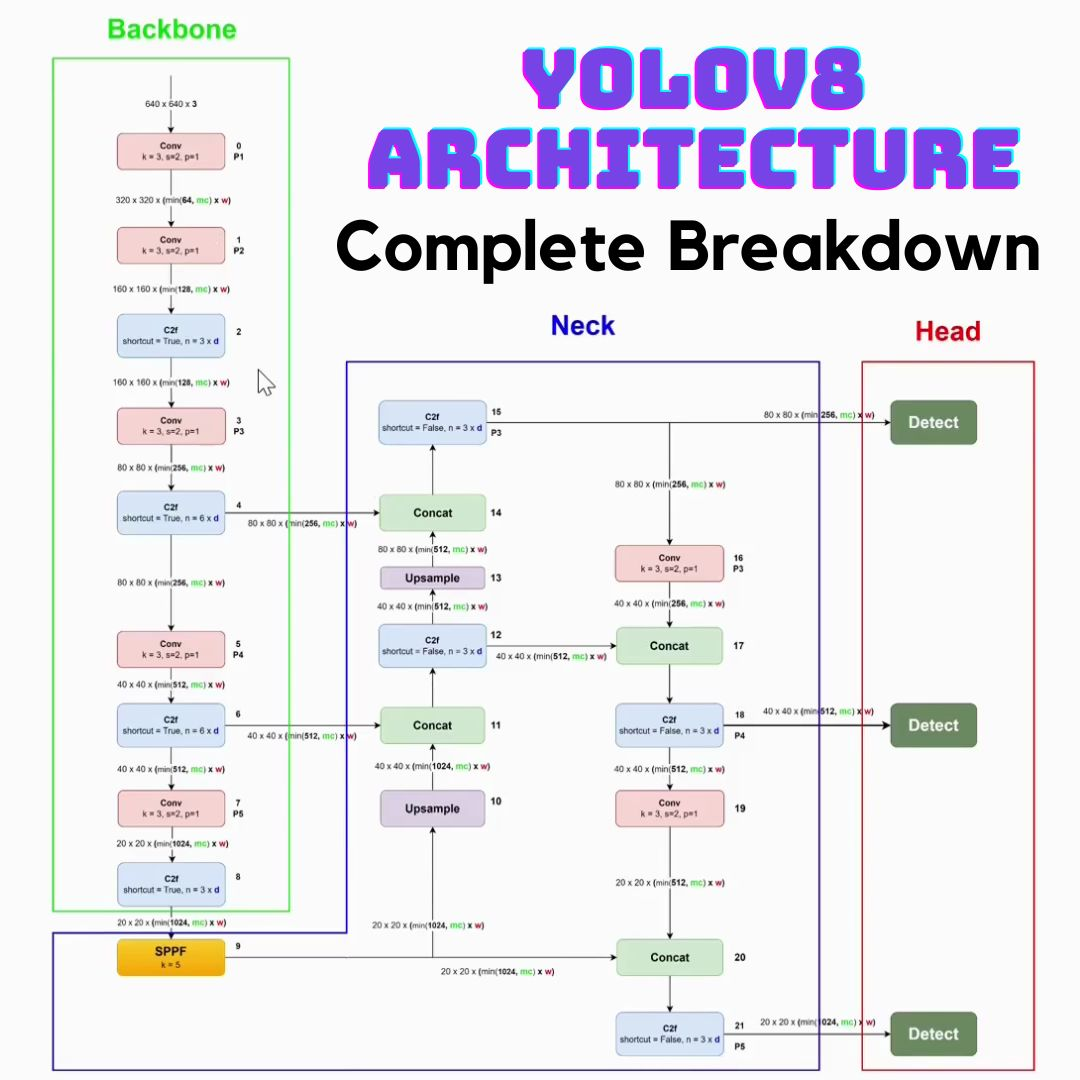
\includegraphics[width=0.55\linewidth]{Figures/1698478493766.jpg}
        \caption{Kiến trúc tổng thể YOLOv8}
    \end{figure}

\end{frame}

\begin{frame}{Hàm mất mát YOLOv8}
    Tối thiểu hóa hàm mất mát tổng hợp:
    $$ L_{total} = \lambda_{box} L_{box} + \lambda_{cls} L_{cls} + \lambda_{dfl} L_{dfl} $$

    \begin{block}{Các thành phần chính}
    \begin{itemize}
        \item \textbf{CIoU Loss ($L_{box}$):} Định vị bounding box
        $$ \mathcal{L}_{CIoU} = 1 - IoU + \frac{\rho^2(\mathbf{b}, \mathbf{b}^{gt})}{c^2} + \alpha v $$
        \item \textbf{Distribution Focal Loss (DFL):} Tối ưu cho box có biên mờ
        \item \textbf{Varifocal Loss ($L_{cls}$):} Cân bằng mẫu khó/dễ
    \end{itemize}
    \end{block}
\end{frame}

%--- BYTETRACK ---
\begin{frame}{Theo dõi đa đối tượng (MOT)}
    \textbf{Mục tiêu:} Gán ID duy nhất cho mỗi đối tượng qua các khung hình liên tiếp

    \begin{block}{Phương pháp: Tracking-by-Detection}
    \begin{itemize}
        \item \textbf{Bộ lọc Kalman:} Ước lượng trạng thái (vị trí, vận tốc) để dự đoán vị trí tiếp theo
        \item \textbf{Thuật toán Hungarian:} Ghép cặp tối ưu giữa \textit{Dự đoán Kalman} và \textit{Phát hiện YOLO}
    \end{itemize}
    \end{block}

    \begin{figure}
        \centering
        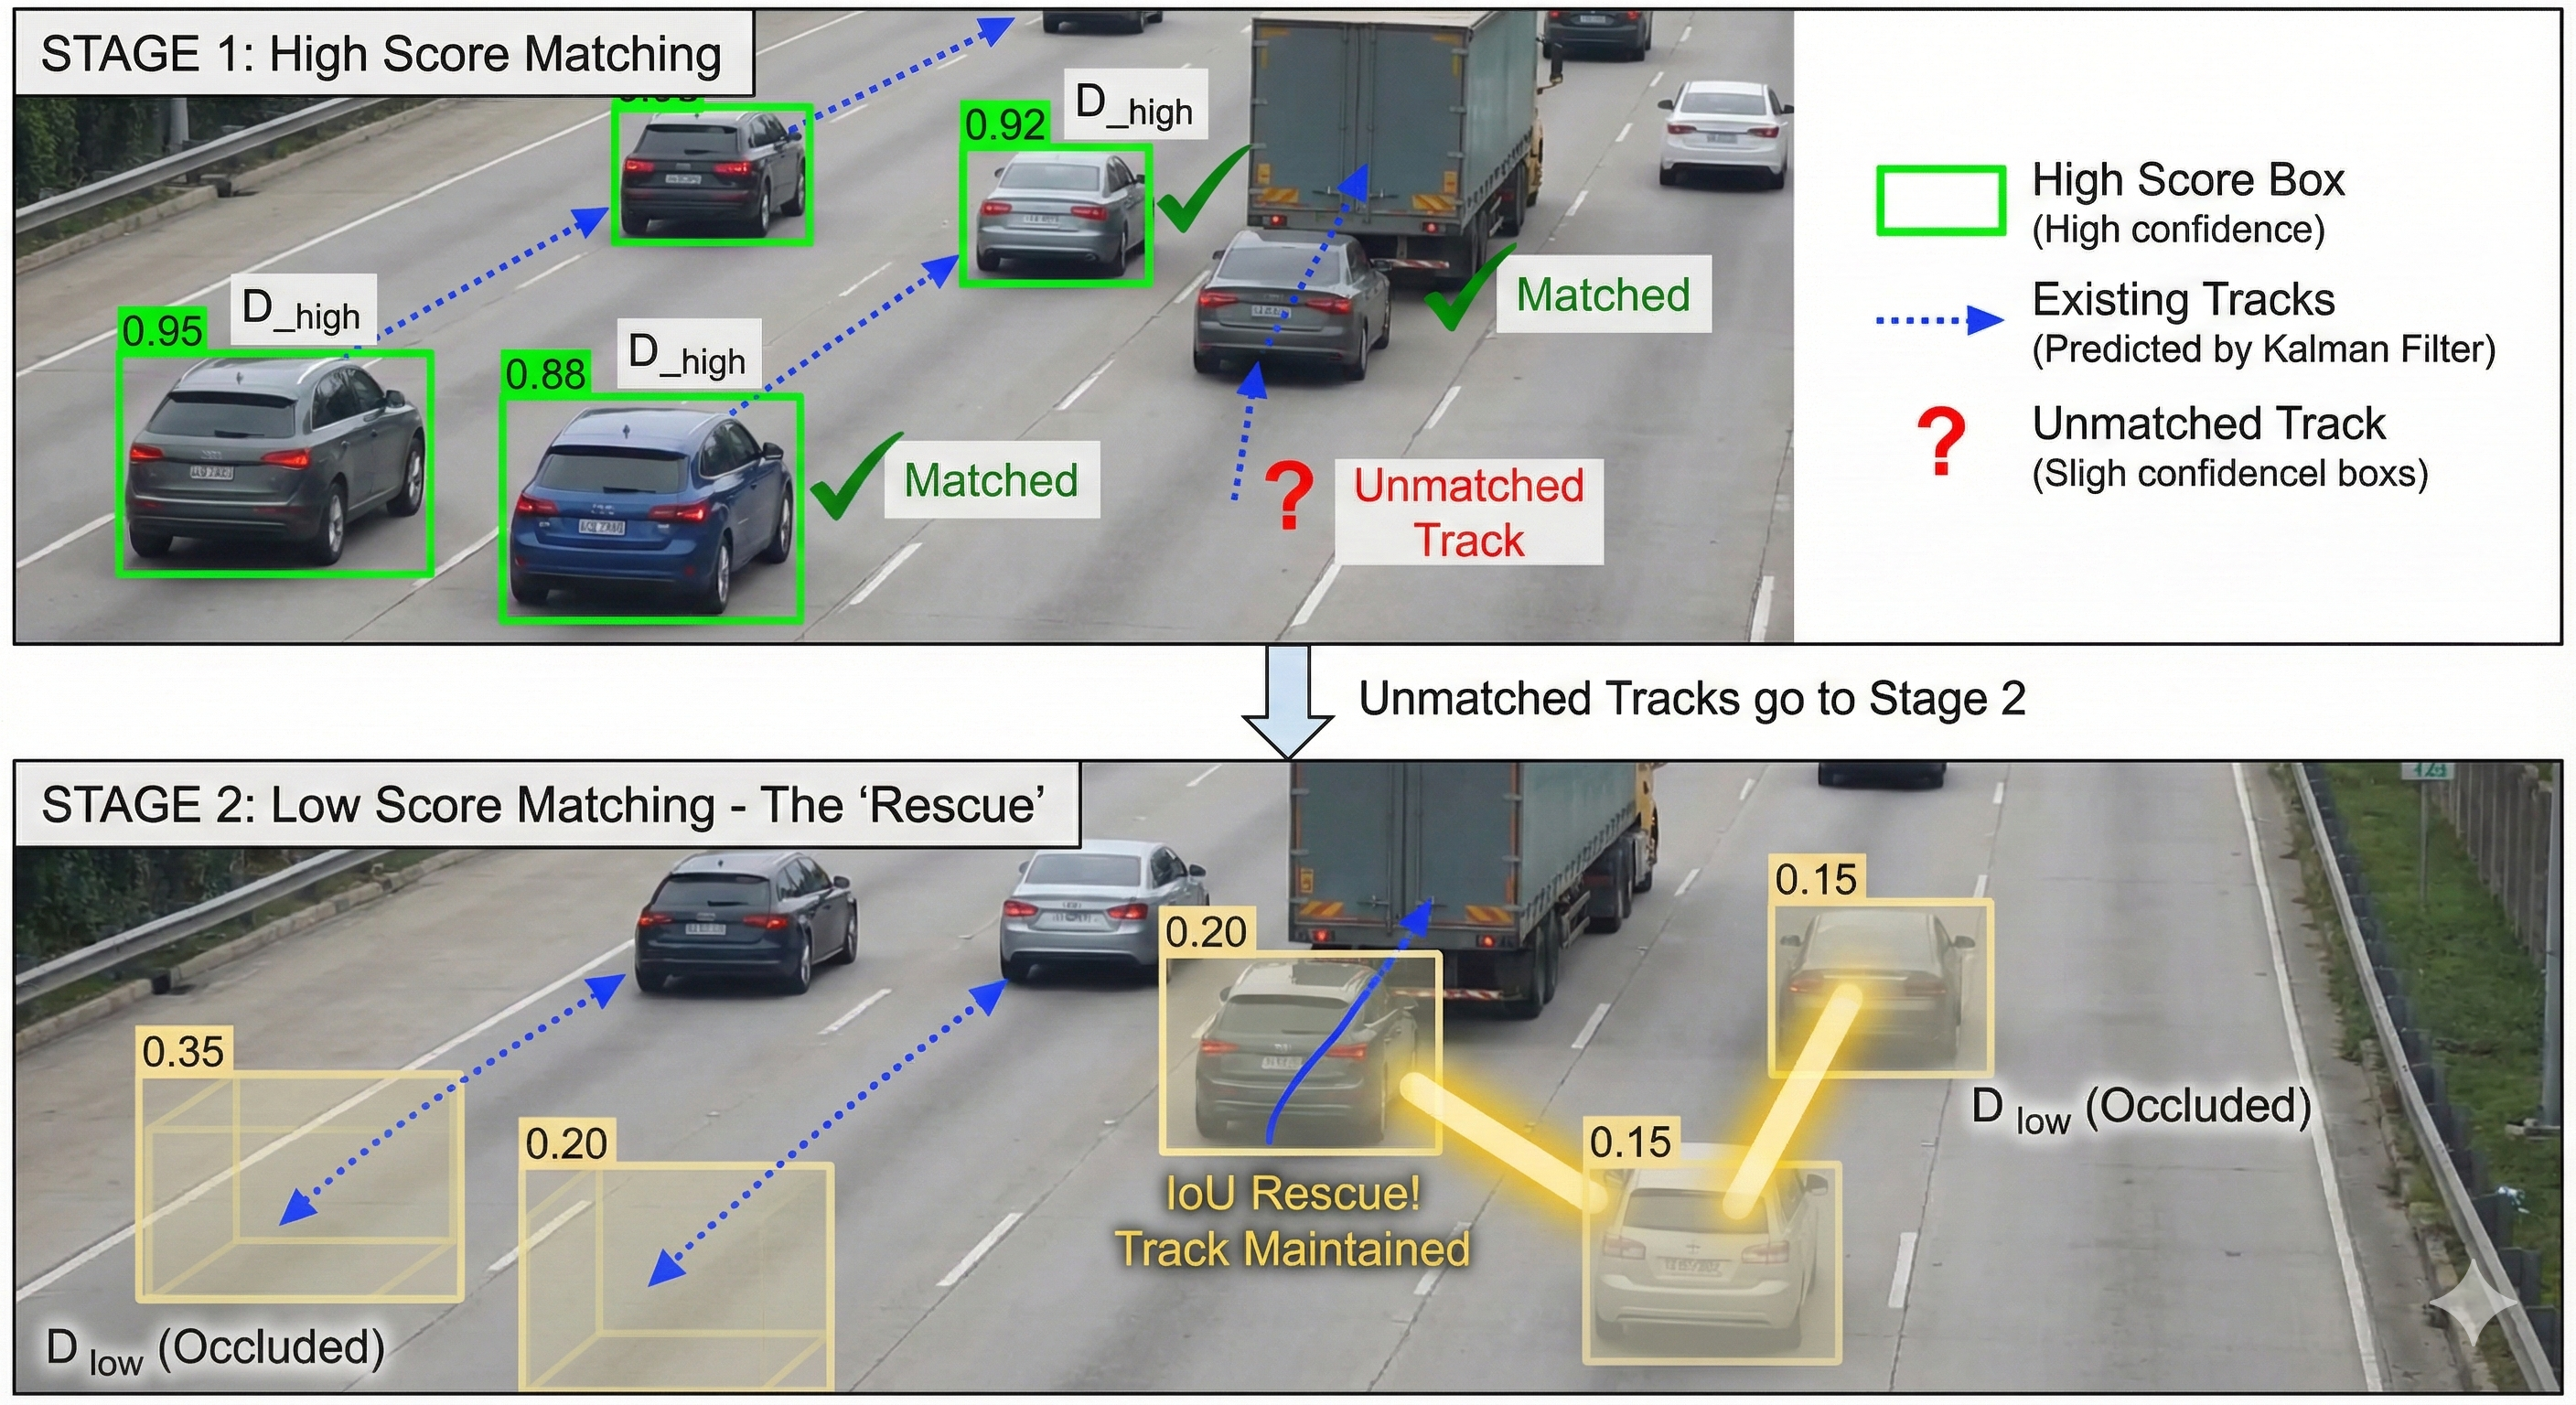
\includegraphics[width=0.5\linewidth]{Figures/bytetrack.png}

    \end{figure}
\end{frame}

\begin{frame}{Thuật toán ByteTrack}
    \textbf{Ý tưởng:} "Tận dụng mọi detection, kể cả độ tin cậy thấp"

    \begin{block}{Quy trình 2 giai đoạn}
    \begin{enumerate}
        \item \textbf{High Score Matching:}
        \begin{itemize}
            \item Ghép detection chất lượng cao ($conf > \tau_{high}$) với Track hiện có
            \item Sử dụng IoU làm trọng số
        \end{itemize}
        \item \textbf{Low Score Matching:}
        \begin{itemize}
            \item Track chưa ghép sẽ tìm trong detection chất lượng thấp ($conf > \tau_{low}$)
            \item "Cứu" lại xe bị che khuất hoặc mờ
        \end{itemize}
    \end{enumerate}
    \end{block}

    \textbf{Ưu điểm:} Tốc độ cao (không cần trích xuất đặc trưng ngoại hình)
\end{frame}

%--- NHẬN DIỆN ĐÈN GIAO THÔNG ---
\begin{frame}{Nhận diện đèn giao thông (HSV)}
    \begin{block}{Chuyển đổi RGB $\rightarrow$ HSV}
    Tách biệt thông tin màu sắc và độ sáng
    \end{block}

    \textbf{Ngưỡng màu cho từng trạng thái đèn:}
    \begin{itemize}
        \item \textbf{Đỏ (Red):} $Hue \in [0, 10] \cup [160, 180]$ (red-wrap effect)
        \item \textbf{Vàng (Yellow):} $Hue \in [15, 35]$
        \item \textbf{Xanh (Green):} $Hue \in [40, 90]$
    \end{itemize}

    \begin{block}{Cơ chế Voting}
    Tính tỷ lệ pixel cho từng mặt nạ màu $\rightarrow$ Xác định trạng thái trội
    \end{block}

    \textit{Hỗ trợ 4 loại đèn: Tròn, Rẽ trái, Rẽ phải, Đi thẳng}
\end{frame}

%--- LOGIC VI PHẠM ---
\begin{frame}{Thuật toán phát hiện Vượt đèn đỏ}
    \begin{block}{Quy trình quyết định (Decision Flow)}
    Khi sự kiện \textit{Stopline Crossing} xảy ra:
    \begin{enumerate}
        \item \textbf{Kiểm tra Quyền đi (Green Priority):}
        \begin{itemize}
            \item Có đèn xanh mũi tên trùng hướng xe? $\rightarrow$ \textcolor{green}{\textbf{HỢP LỆ}}
        \end{itemize}

        \item \textbf{Kiểm tra Cấm (Red Constraint):}
        \begin{itemize}
            \item Đèn đỏ tròn hoạt động? HOẶC Đèn đỏ mũi tên trùng hướng xe?
            \item $\rightarrow$ Nếu Đúng: \textcolor{red}{\textbf{VI PHẠM}}
        \end{itemize}

        \item \textbf{Xác nhận:} Loại trừ ngoại lệ (xe ưu tiên)
    \end{enumerate}
    \end{block}
\end{frame}

\begin{frame}{Thuật toán phát hiện Đi sai làn}
    \textbf{Cấu hình Lane Manager:}
    \begin{itemize}
        \item Mỗi làn là một \textit{Polygon} + danh sách \texttt{allowed\_classes}
        \item Hỗ trợ làn đè (overlapping lanes)
    \end{itemize}

    \begin{block}{Quy trình kiểm tra}
    \begin{enumerate}
        \item Tính tọa độ tâm $(C_x, C_y)$ của xe từ Bounding Box
        \item \textbf{Point-in-Polygon Test:} Xác định xe thuộc làn $L_i$ nào
        \item \textbf{Class Verification:}
        $$ \text{Violation} = (C \in L_i) \land (Class_v \notin L_i.allowed) $$
    \end{enumerate}
    \end{block}

    \textit{Sử dụng Ray Casting Algorithm cho Point-in-Polygon}
\end{frame}

%============================================================
% PHẦN MỚI: LÝ THUYẾT ALPR VÀ OCR
%============================================================
\begin{frame}{Tổng quan ALPR (Nhận diện biển số)}
    \textbf{ALPR = Automatic License Plate Recognition}

    \begin{block}{Pipeline tổng quát}
    \centering
    \begin{tikzpicture}[
        scale=0.8, transform shape,
        node distance=0.3cm and 0.4cm,
        box/.style={rectangle, draw, rounded corners, minimum width=1.5cm, minimum height=0.5cm, align=center, font=\tiny},
        arrow/.style={->, thick, >=stealth}
    ]
        \node[box, fill=blue!20] (input) {Ảnh\\đầu vào};
        \node[box, fill=orange!20, right=of input] (detect) {Plate\\Detection};
        \node[box, fill=yellow!20, right=of detect] (preprocess) {Tiền xử lý\\(CLAHE)};
        \node[box, fill=green!20, right=of preprocess] (ocr) {OCR};
        \node[box, fill=purple!20, right=of ocr] (output) {Biển số};

        \draw[arrow] (input) -- (detect);
        \draw[arrow] (detect) -- (preprocess);
        \draw[arrow] (preprocess) -- (ocr);
        \draw[arrow] (ocr) -- (output);
    \end{tikzpicture}
    \end{block}

    \textbf{Thách thức nhận diện biển số Việt Nam:}
    \begin{itemize}
        \item Đa dạng định dạng: 1 dòng, 2 dòng
        \item Điều kiện thực tế: Bẩn, mờ, nghiêng
        \item Ánh sáng: Phản chiếu, bóng đổ
    \end{itemize}
\end{frame}

\begin{frame}{Biển số xe Việt Nam}
    \begin{table}
        \centering
        \small
        \begin{tabular}{|c|l|l|}
            \hline
            \textbf{Loại} & \textbf{Định dạng} & \textbf{Ví dụ} \\
            \hline
            Xe ô tô (1 dòng) & XX-Y XXXXX & 30G-07784 \\
            \hline
            Xe ô tô (2 dòng) & XX-Y / XXXXX & 30G / 07784 \\
            \hline
            Xe máy & XX-YZ / XXX.XX & 29-H1 / 234.56 \\
            \hline
        \end{tabular}
    \end{table}

    \textbf{Cấu trúc:}
    \begin{itemize}
        \item \textbf{2 số đầu:} Mã tỉnh (30 = Hà Nội, 51 = TP.HCM)
        \item \textbf{1 chữ cái:} Seri (A-Z, trừ I, O, Q)
        \item \textbf{5 số cuối:} Số thứ tự đăng ký
    \end{itemize}
\end{frame}

%--- PADDLEOCR ---
\begin{frame}{PaddleOCR - Kiến trúc CRNN}
    \textbf{CRNN = Convolutional Recurrent Neural Network}

    \begin{block}{3 thành phần chính}
    \begin{enumerate}
        \item \textbf{CNN Backbone:} Trích xuất đặc trưng không gian từ ảnh
        \begin{itemize}
            \item Sử dụng MobileNet/ResNet biến thể
        \end{itemize}
        \item \textbf{Sequence Modeling (Bi-LSTM):}
        \begin{itemize}
            \item Mô hình hóa quan hệ tuần tự giữa các ký tự
            \item Bidirectional: capture thông tin cả 2 hướng
        \end{itemize}
        \item \textbf{CTC Decoder:} Giải mã chuỗi ký tự cuối cùng
    \end{enumerate}
    \end{block}

    \centering
    \small
    Ảnh biển số $\rightarrow$ CNN $\rightarrow$ Bi-LSTM $\rightarrow$ CTC $\rightarrow$ ``30G07784''
\end{frame}

\begin{frame}{CTC Loss (Connectionist Temporal Classification)}
    \textbf{Đặc điểm:} Huấn luyện không cần alignment giữa input và output

    \begin{block}{Công thức}
    Xác suất của chuỗi output $\mathbf{l}$:
    $$ P(\mathbf{l} | \mathbf{x}) = \sum_{\pi \in \mathcal{B}^{-1}(\mathbf{l})} P(\pi | \mathbf{x}) $$

    CTC Loss = Negative log-likelihood:
    $$ \mathcal{L}_{CTC} = -\log P(\mathbf{l} | \mathbf{x}) $$
    \end{block}

    \textbf{Ví dụ:} Chuỗi mục tiêu ``AB''
    \begin{itemize}
        \item ``A-A-B-B'' $\rightarrow$ ``AB'' (loại bỏ ký tự lặp)
        \item ``A--B-'' $\rightarrow$ ``AB'' (loại bỏ blank `-')
    \end{itemize}
\end{frame}

%--- TIỀN XỬ LÝ ---
\begin{frame}{CLAHE - Cân bằng histogram thích ứng}
    \textbf{CLAHE = Contrast Limited Adaptive Histogram Equalization}

    \begin{block}{Nguyên lý hoạt động}
    \begin{enumerate}
        \item \textbf{Chia tile:} Chia ảnh thành các tile nhỏ (8×8 pixels)
        \item \textbf{HE cục bộ:} Histogram Equalization trên từng tile
        \item \textbf{Clip Limit:} Giới hạn độ tương phản (tránh khuếch đại noise)
        $$ \beta = \frac{M \times N}{L} \times \text{clipLimit} $$
        \item \textbf{Bilinear Interpolation:} Ghép các tile mượt mà
    \end{enumerate}
    \end{block}

    \textbf{Cấu hình:} \texttt{clipLimit=2.0}, \texttt{tileGridSize=(8,8)}
\end{frame}

\begin{frame}{Sharpening - Làm sắc nét}
    \textbf{Mục đích:} Tăng cường cạnh ký tự trước khi đưa vào OCR

    \begin{block}{Kernel Sharpening}
    $$ K_{sharpen} = \begin{bmatrix} 0 & -1 & 0 \\ -1 & 5 & -1 \\ 0 & -1 & 0 \end{bmatrix} $$
    \end{block}

    \textbf{Công thức pixel mới:}
    $$ I'(x,y) = 5 \cdot I(x,y) - [I(x-1,y) + I(x+1,y) + I(x,y-1) + I(x,y+1)] $$

    \textit{Tăng cường sự khác biệt giữa pixel và các pixel xung quanh \\  $\rightarrow$ Cạnh sắc nét hơn}
\end{frame}

%--- VALIDATION & RETRY ---
\begin{frame}{Character Correction - Hiệu chỉnh ký tự}
    \textbf{Vấn đề:} OCR có thể nhầm lẫn ký tự tương tự

    \begin{table}
        \centering
        \small
        \begin{tabular}{|c|c|l|}
            \hline
            \textbf{Sai} & \textbf{Đúng} & \textbf{Điều kiện} \\
            \hline
            0 (số) & O (chữ) & Vị trí chữ cái (index 2) \\
            \hline
            O (chữ) & 0 (số) & Vị trí chữ số \\
            \hline
            1 (số) & I (chữ) & Vị trí chữ cái \\
            \hline
            8 (số) & B (chữ) & Vị trí chữ cái \\
            \hline
        \end{tabular}
    \end{table}

    \textbf{Logic hiệu chỉnh theo định dạng VN:}
    \begin{itemize}
        \item Vị trí 0-1: Bắt buộc chữ số (mã tỉnh)
        \item Vị trí 2: Bắt buộc chữ cái (seri)
        \item Vị trí 3+: Bắt buộc chữ số
    \end{itemize}
\end{frame}

\begin{frame}{Format Validation \& Retry Mechanism}
    \textbf{Vấn đề:} OCR có thể cho kết quả khác nhau giữa các frame
    \begin{itemize}
        \item Biển số bị rung, blur khi xe di chuyển
        \item Ánh sáng thay đổi, góc nhìn thay đổi
    \end{itemize}

    \begin{block}{Giải pháp: Format Validation}
    Validate theo định dạng biển số Việt Nam:
    \begin{itemize}
        \item \textbf{Xe máy:} \texttt{[0-9]\{2\}[A-Z][A-Z0-9][0-9]\{4,5\}} (8-9 ký tự)
        \item \textbf{Ô tô:} \texttt{[0-9]\{2\}[A-Z][0-9]\{4,5\}} (7-8 ký tự)
    \end{itemize}
    \end{block}

    \textbf{Retry Mechanism:}
    \begin{itemize}
        \item Sai format $\rightarrow$ không lưu, thử lại frame sau
        \item Đã có kết quả valid $\rightarrow$ dừng OCR (tiết kiệm tài nguyên)
    \end{itemize}
\end{frame}

%--- HƯỚNG DI CHUYỂN ---
\begin{frame}{Xác định hướng di chuyển}
    \textbf{Direction Fusion - Kết hợp 2 nguồn:}

    \begin{columns}
        \column{0.5\textwidth}
        \begin{block}{Nguồn 1: Trajectory}
        \begin{itemize}
            \item Tính vector chuyển động từ lịch sử vị trí
            \item So sánh với Reference Vector
            \item Khử nghiêng camera
        \end{itemize}
        \end{block}

        \column{0.5\textwidth}
        \begin{block}{Nguồn 2: ROI-based}
        \begin{itemize}
            \item Xác định hướng dựa trên vùng xe đang đi qua
            \item Cấu hình sẵn cho từng làn
        \end{itemize}
        \end{block}
    \end{columns}

    \vspace{0.5em}
    \textbf{Góc lệch:}
    $$ \alpha = \operatorname{atan2}(\vec{v} \times \vec{r}, \ \vec{v} \cdot \vec{r}) $$

    Trong đó $\vec{v}$: vector chuyển động xe, $\vec{r}$: vector tham chiếu đường
\end{frame}

%----------------------------------------------------------------------------------------
%   PHẦN 3: PHƯƠNG PHÁP TRIỂN KHAI
%----------------------------------------------------------------------------------------
\section{Phương pháp triển khai}

\begin{frame}{Tóm tắt các mô hình sử dụng}
    \begin{table}
        \centering
        \small
        \begin{tabular}{|l|l|l|}
            \hline
            \textbf{Thành phần} & \textbf{Mô hình} & \textbf{Vai trò} \\
            \hline
            Phát hiện xe & YOLOv8n & 5 lớp phương tiện \\
            \hline
            Phát hiện biển số & YOLOv8n & 1 lớp (plate) \\
            \hline
            Mô hình tích hợp & YOLOv8n & 6 lớp (5 xe + plate) \\
            \hline
            Tracking & ByteTrack & Theo dõi đa đối tượng \\
            \hline
            OCR & PaddleOCR + CLAHE & Nhận dạng ký tự biển số \\
            \hline
        \end{tabular}
        \caption{Tổng hợp các mô hình trong hệ thống}
    \end{table}


\end{frame}

%--- SƠ ĐỒ PIPELINE 1 ---
\begin{frame}{Pipeline 1: Sơ đồ triển khai (Two-Stage)}
    \centering
    \begin{tikzpicture}[
        scale=0.95, transform shape,
        node distance=0.5cm and 0.6cm,
        box/.style={rectangle, draw, rounded corners, minimum width=2cm, minimum height=0.7cm, align=center, font=\scriptsize},
        arrow/.style={->, thick, >=stealth}
    ]
        % Row 1
        \node[box, fill=blue!20] (frame) {Frame};
        \node[box, fill=orange!20, right=of frame] (yolo1) {YOLOv8n\\(5 lớp xe)};
        \node[box, fill=yellow!20, right=of yolo1] (track) {ByteTrack};
        \node[box, fill=green!20, right=of track] (crop) {Crop xe};

        % Row 2
        \node[box, fill=red!20, below=1cm of crop] (yolo2) {YOLOv8n\\(plate)};
        \node[box, fill=purple!20, left=of yolo2] (clahe) {CLAHE};
        \node[box, fill=cyan!20, left=of clahe] (ocr) {PaddleOCR};
        \node[box, fill=gray!20, left=of ocr] (valid) {Validation};

        % Arrows Row 1
        \draw[arrow] (frame) -- (yolo1);
        \draw[arrow] (yolo1) -- (track);
        \draw[arrow] (track) -- (crop);

        % Arrow down
        \draw[arrow] (crop) -- (yolo2);

        % Arrows Row 2
        \draw[arrow] (yolo2) -- (clahe);
        \draw[arrow] (clahe) -- (ocr);
        \draw[arrow] (ocr) -- (valid);

        % Labels
        \node[above=0.15cm of yolo1, font=\scriptsize, text=blue] {Detect};
    \end{tikzpicture}

    \vspace{0.3em}
\end{frame}

%--- SƠ ĐỒ PIPELINE 2 ---
\begin{frame}{Pipeline 2: Sơ đồ triển khai (One-Stage)}
    \centering
    \begin{tikzpicture}[
        scale=0.8, transform shape,
        node distance=0.5cm and 0.5cm,
        box/.style={rectangle, draw, rounded corners, minimum width=1.8cm, minimum height=0.7cm, align=center, font=\scriptsize},
        arrow/.style={->, thick, >=stealth}
    ]
        % Row 1: Input and detection
        \node[box, fill=blue!20] (frame) {Frame};
        \node[box, fill=orange!20, right=0.7cm of frame] (yolo) {YOLOv8n\\(6 lớp)};
        \node[box, fill=yellow!20, above right=0.4cm and 0.7cm of yolo] (vehicles) {Vehicles};
        \node[box, fill=green!20, below right=0.4cm and 0.7cm of yolo] (plates) {Plates};
        \node[box, fill=teal!20, right=1.6cm of yolo] (match) {Matching};

        % Row 2: OCR pipeline
        \node[box, fill=purple!20, right=0.6cm of match] (clahe) {CLAHE};
        \node[box, fill=cyan!20, right=of clahe] (ocr) {PaddleOCR};
        \node[box, fill=gray!20, right=of ocr] (valid) {Validation};

        % Arrows
        \draw[arrow] (frame) -- (yolo);
        \draw[arrow] (yolo) -- (vehicles);
        \draw[arrow] (yolo) -- (plates);
        \draw[arrow] (vehicles) -- (match);
        \draw[arrow] (plates) -- (match);
        \draw[arrow] (match) -- (clahe);
        \draw[arrow] (clahe) -- (ocr);
        \draw[arrow] (ocr) -- (valid);

        % Labels
        \node[above=0.15cm of yolo, font=\scriptsize, text=red] {1 inference};
        \node[above=0.15cm of match, font=\scriptsize, text=blue] {plate $\in$ xe?};
    \end{tikzpicture}

    \vspace{0.3em}
\end{frame}

\begin{frame}{Pipeline ALPR chi tiết}
    \begin{block}{Quy trình nhận diện biển số (Pipeline 1)}
    \begin{enumerate}
        \item \textbf{Plate Detection:} YOLOv8n phát hiện vùng biển số
        \item \textbf{Tiền xử lý ảnh:}
        \begin{itemize}
            \item CLAHE (Contrast Limited Adaptive Histogram Equalization)
            \item Grayscale conversion
            \item Noise reduction
        \end{itemize}
        \item \textbf{OCR:} PaddleOCR nhận dạng ký tự
        \item \textbf{Hậu xử lý:}
        \begin{itemize}
            \item Character correction (0$\leftrightarrow$O, 1$\leftrightarrow$I)
            \item Format validation (biển số Việt Nam)
        \end{itemize}
    \end{enumerate}
    \end{block}
\end{frame}

\begin{frame}{Cấu hình huấn luyện}
    \begin{table}
        \centering
        \begin{tabular}{|l|c|c|c|}
            \hline
            \textbf{Tham số} & \textbf{Model 1} & \textbf{Model 2} & \textbf{Tích hợp} \\
            \hline
            Base Model & YOLOv8n & YOLOv8n & YOLOv8n \\
            \hline
            Số lớp & 5 (xe) & 1 (plate) & 6 \\
            \hline
            Image Size & 416×416 & 416×416 & 640×640 \\
            \hline
            Batch Size & 16 & 16 & 64 \\
            \hline
            Epochs & 100 & 100 & 100 \\
            \hline
            Optimizer & SGD & AdamW & SGD \\
            \hline
        \end{tabular}
        \caption{Cấu hình huấn luyện 3 mô hình}
    \end{table}
\end{frame}

\begin{frame}{Dữ liệu huấn luyện}
    \begin{columns}
        \column{0.5\textwidth}
        \textbf{Dataset phát hiện xe:}
        \begin{itemize}
            \item Nguồn: CCTV + Camera thực tế
            \item Quy mô: >16,000 ảnh
            \item Labels: >65,000 boxes
            \item 5 lớp: ô tô, xe máy, xe buýt, xe tải, xe đạp
        \end{itemize}

        \column{0.5\textwidth}
        \textbf{Dataset biển số (VNLP):}
        \begin{itemize}
            \item Nguồn: Thu thập thực tế
            \item Đa dạng: Nhiều góc độ, ánh sáng
            \item Biển số Việt Nam: 1 hàng, 2 hàng
            \item Fine-tuned từ pretrained weights
        \end{itemize}
    \end{columns}

    \vspace{1em}
    \begin{figure}
        \centering
        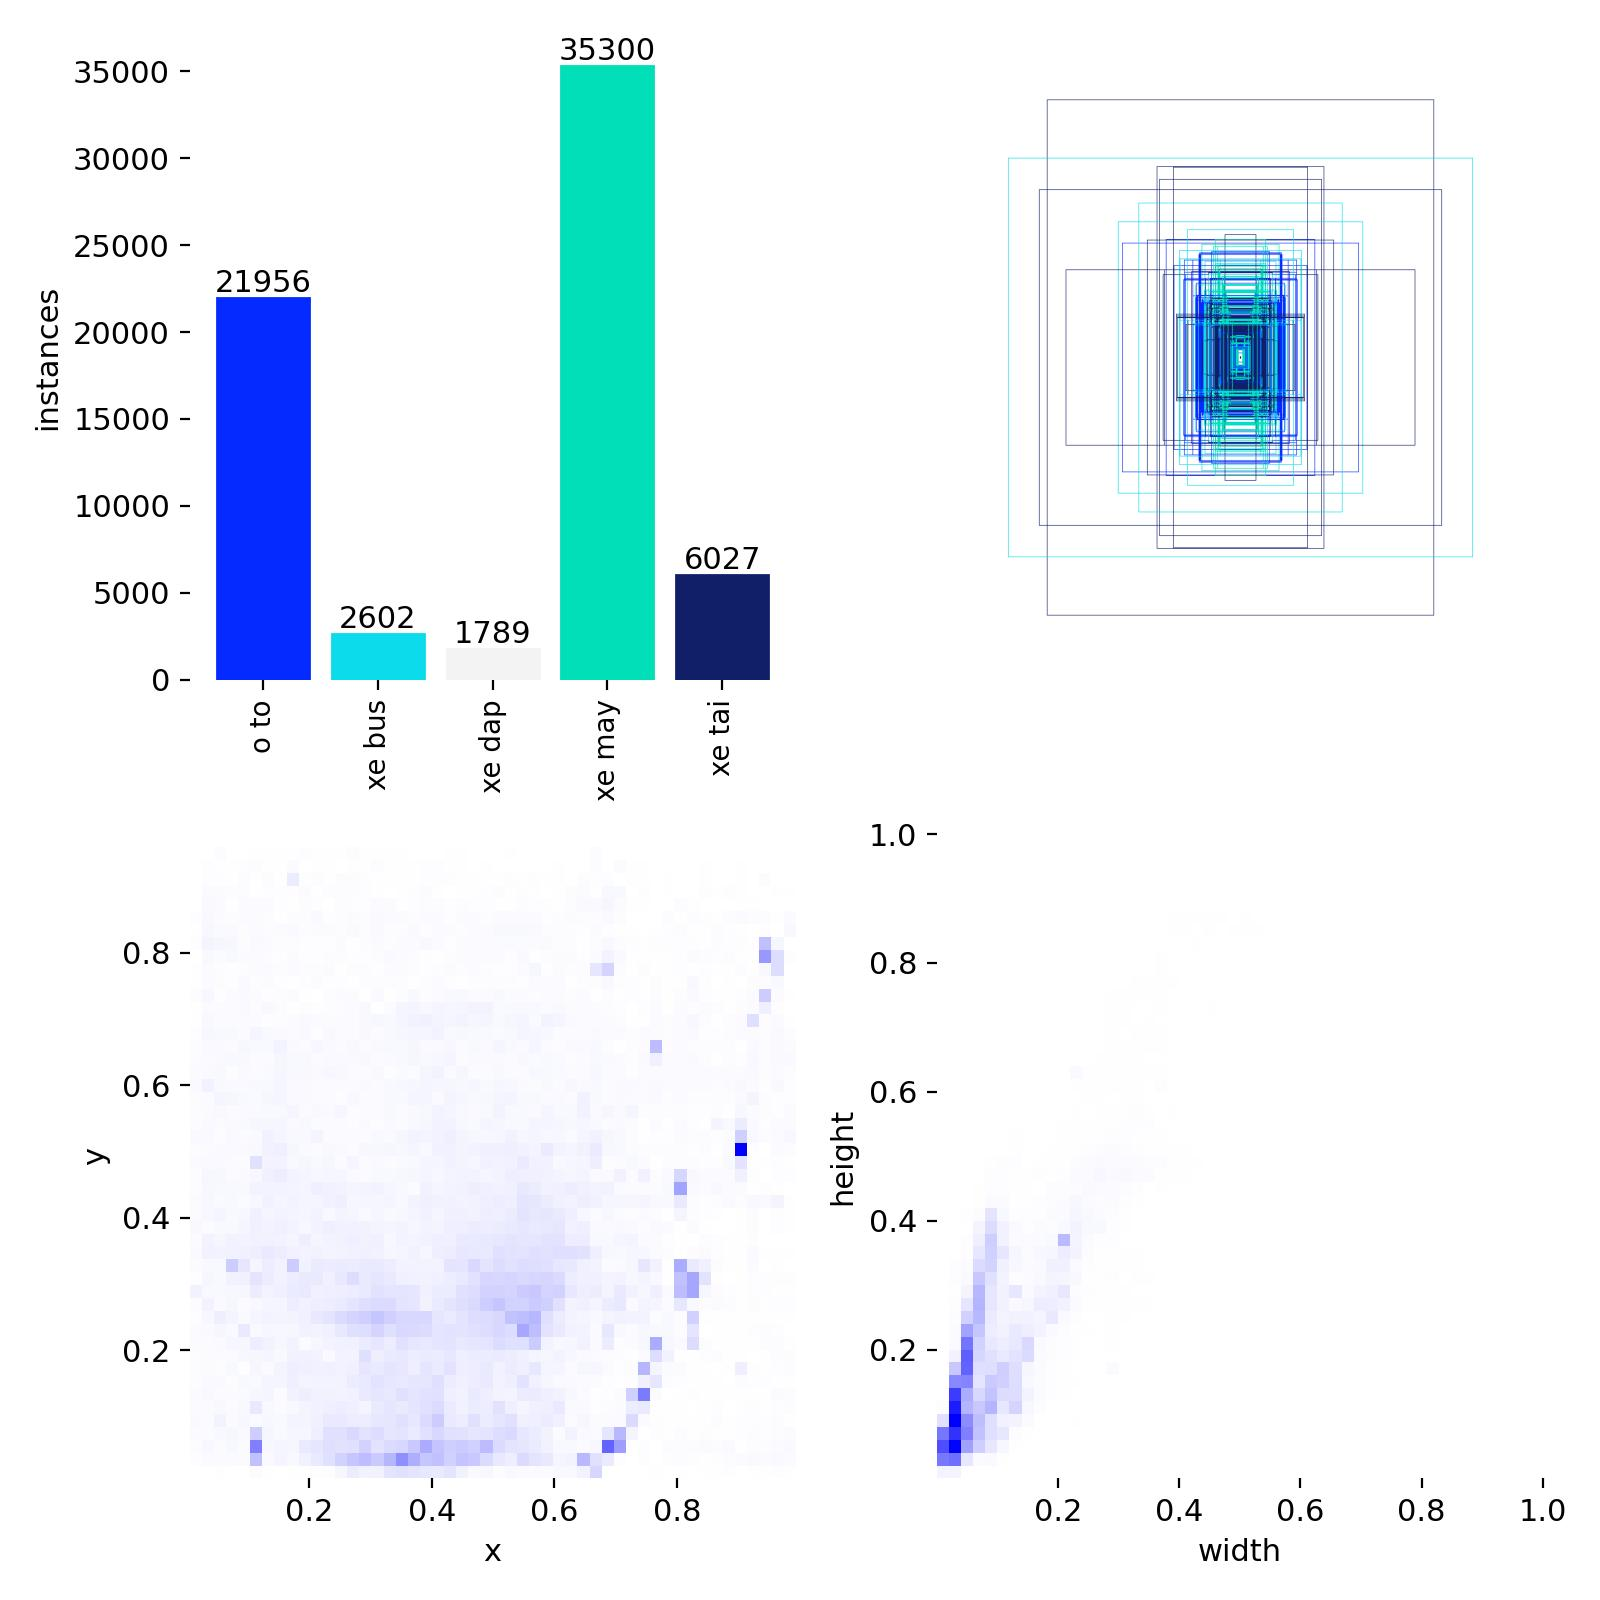
\includegraphics[width=0.5\linewidth]{Figures/labels.jpg}
        \caption{Phân bố nhãn trong dataset phương tiện}
    \end{figure}
\end{frame}

%--- PIPELINE 2 CHI TIẾT ---
\begin{frame}{Pipeline 2: Mô hình tích hợp 6 lớp}
    \begin{block}{Ý tưởng: Huấn luyện 1 model phát hiện đồng thời xe và biển số}
    \begin{enumerate}
        \item Frame $\rightarrow$ YOLOv8n (6 lớp) $\rightarrow$ \{Vehicles, Plates\}
        \item \textbf{Matching:} Kiểm tra Plate nằm trong Vehicle (Containment)
        \item Crop biển số $\rightarrow$ CLAHE $\rightarrow$ PaddleOCR
        \item Format Validation + Retry
    \end{enumerate}
    \end{block}

    \textbf{Ưu điểm so với Pipeline 1:}
    \begin{itemize}
        \item Chỉ 1 lần forward pass qua YOLO (nhanh hơn 2--3x)
        \item Mapping plate$\rightarrow$xe tự động qua containment check
        \item Tiết kiệm GPU Memory (~1.2GB vs ~2.5GB)
        \item Model học được mối quan hệ không gian xe--biển số
    \end{itemize}
\end{frame}

%--- TẠO DỮ LIỆU PIPELINE 2 ---
\begin{frame}{Tạo dữ liệu cho Pipeline 2: Vấn đề}
    \begin{alertblock}{Vấn đề}
    \begin{itemize}
        \item Dataset phương tiện (vietnam\_vehicle\_dataset): \textbf{chỉ có 5 lớp xe}
        \item Dataset biển số (VNLP): \textbf{chỉ có 1 lớp plate}
        \item \textbf{Cần:} Dataset 6 lớp (5 xe + plate) để huấn luyện model tích hợp
    \end{itemize}
    \end{alertblock}

    \begin{block}{Giải pháp: Semi-supervised Labeling}
    Sử dụng Model 2 (đã train trên VNLP, mAP 99.5\%) làm \textbf{Teacher Model} để tự động gán nhãn biển số cho dataset xe
    \end{block}
\end{frame}

\begin{frame}{Tạo dữ liệu Pipeline 2: Quy trình chi tiết}
    \centering
    \begin{tikzpicture}[
        scale=0.8, transform shape,
        node distance=0.3cm and 0.5cm,
        box/.style={rectangle, draw, rounded corners, minimum width=2cm, minimum height=0.6cm, align=center, font=\tiny},
        arrow/.style={->, thick, >=stealth}
    ]
        % Row 1
        \node[box, fill=blue!20] (dataset) {Dataset xe\\(5 lớp)};
        \node[box, fill=orange!20, right=of dataset] (teacher) {Teacher Model\\(mAP 99.5\%)};
        \node[box, fill=green!20, right=of teacher] (infer) {Inference\\toàn bộ ảnh};
        \node[box, fill=yellow!20, right=of infer] (detect) {Phát hiện\\bbox plate};
        \node[box, fill=purple!20, right=of detect] (merge) {Merge\\annotation};
        \node[box, fill=cyan!20, right=of merge] (result) {Dataset\\6 lớp};

        % Arrows
        \draw[arrow] (dataset) -- (teacher);
        \draw[arrow] (teacher) -- (infer);
        \draw[arrow] (infer) -- (detect);
        \draw[arrow] (detect) -- (merge);
        \draw[arrow] (merge) -- (result);
    \end{tikzpicture}

    \vspace{0.5em}
    \begin{block}{Các bước chi tiết}
    \begin{enumerate}
        \item \textbf{Chuẩn bị:} Dataset xe (16,000+ ảnh, 5 lớp) + Teacher Model (YOLOv8n)
        \item \textbf{Inference:} Chạy Teacher trên từng ảnh $\rightarrow$ Phát hiện bbox biển số
        \item \textbf{Lọc:} Chỉ giữ bbox có confidence > 0.5
        \item \textbf{Merge:} Thêm bbox plate (class\_id = 5) vào file annotation gốc
        \item \textbf{Kết quả:} Dataset 6 lớp (5 xe + 1 plate) sẵn sàng huấn luyện
    \end{enumerate}
    \end{block}
\end{frame}

\begin{frame}{Tạo dữ liệu Pipeline 2}


    \begin{alertblock}{Lưu ý}
    \begin{itemize}
        \item Chỉ thêm bbox có confidence > 0.5
        \item Không xóa nhãn xe gốc (5 lớp)
        \item Kết quả: ~65,000 boxes xe + ~X boxes plate
    \end{itemize}
    \end{alertblock}
\end{frame}

\begin{frame}{Pipeline 2: Trade-off sau khi huấn luyện}
    \begin{table}
        \centering
        \small
        \begin{tabular}{|l|c|c|}
            \hline
            \textbf{Metric} & \textbf{Model 2 (VNLP)} & \textbf{Model tích hợp} \\
            \hline
            Số lớp & 1 (plate) & 6 (5 xe + plate) \\
            \hline
            mAP@50 (plate) & \textbf{99.5\%} & 59\% \\
            \hline
            Tốc độ (FPS) & -- & 15--20 FPS \\
            \hline
            GPU Memory & ~0.8GB & ~1.2GB \\
            \hline
        \end{tabular}
    \end{table}

    \textbf{Nguyên nhân mAP plate giảm:}
    \begin{itemize}
        \item \textbf{Class imbalance:} Số lượng xe >> số lượng biển số
        \item \textbf{Kích thước nhỏ:} Biển số chiếm diện tích rất nhỏ trong ảnh
        \item \textbf{Annotation noise:} Gán nhãn tự động có thể bỏ sót biển mờ/nhỏ
    \end{itemize}
\end{frame}

\begin{frame}{Pipeline 2: Gán nhãn bán giám sát (Semi-supervised)}
    \textbf{Vấn đề:} Dataset xe (5 lớp) không có nhãn biển số

    \begin{block}{Quy trình gán nhãn tự động}
    \begin{enumerate}
        \item \textbf{Teacher Model:} Dùng Model 2 (mAP 99.5\%) đã huấn luyện
        \item \textbf{Inference:} Chạy Teacher trên toàn bộ ảnh dataset xe
        \item \textbf{Merge:} Thêm bbox biển số vào annotation gốc
        \item \textbf{Kết quả:} Dataset 6 lớp (5 xe + 1 plate)
    \end{enumerate}
    \end{block}

    \begin{alertblock}{Trade-off}
    mAP plate giảm từ 99.5\% xuống 59\% do:
    \begin{itemize}
        \item Class imbalance (biển số ít hơn nhiều so với xe)
        \item Kích thước biển số nhỏ trong image size 416px
    \end{itemize}
    \end{alertblock}
\end{frame}

%--- TIỀN XỬ LÝ OCR ---
\begin{frame}{Tiền xử lý ảnh biển số}
    \begin{columns}
        \column{0.5\textwidth}
        \textbf{Bước 1: CLAHE}
        \begin{itemize}
            \item Cải thiện độ tương phản
            \item clipLimit = 2.0
            \item tileGridSize = (8, 8)
            \item Hiệu quả với ảnh tối/sáng không đều
        \end{itemize}

        \column{0.5\textwidth}
        \textbf{Bước 2: Sharpening}
        $$ K = \begin{bmatrix} 0 & -1 & 0 \\ -1 & 5 & -1 \\ 0 & -1 & 0 \end{bmatrix} $$
        Làm sắc nét cạnh ký tự
    \end{columns}

    \vspace{0.5em}
    \begin{block}{Character Correction}
    Hiệu chỉnh theo vị trí trong biển số:
    \begin{itemize}
        \item Vị trí 0-1: Chữ số (mã tỉnh) $\rightarrow$ O $\rightarrow$ 0
        \item Vị trí 2: Chữ cái (seri) $\rightarrow$ 0 $\rightarrow$ O
        \item Vị trí 3+: Chữ số $\rightarrow$ B $\rightarrow$ 8
    \end{itemize}
    \end{block}
\end{frame}

%--- FORMAT VALIDATION ---
\begin{frame}{Validation biển số Việt Nam}
    \begin{block}{Định dạng biển số hợp lệ}
    \begin{itemize}
        \item \textbf{Xe máy:} xxYZxxxxx (8-9 ký tự)
        \begin{itemize}
            \item xx: Mã tỉnh (2 số)
            \item Y: Seri (1 chữ)
            \item Z: Số/chữ
            \item xxxxx: 4-5 số cuối
            \item VD: \texttt{29B12345}, \texttt{30M04019}
        \end{itemize}
        \item \textbf{Ô tô:} xxYxxxxx (7-8 ký tự)
        \begin{itemize}
            \item VD: \texttt{51A1234}, \texttt{30H12345}
        \end{itemize}
    \end{itemize}
    \end{block}

    \textbf{Retry Mechanism:}
    \begin{itemize}
        \item Chỉ lưu kết quả đúng format (validated)
        \item Sai format $\rightarrow$ retry frame tiếp theo
        \item Đã có kết quả valid $\rightarrow$ dừng OCR cho xe đó
    \end{itemize}
\end{frame}

%----------------------------------------------------------------------------------------
%   PHẦN 4: KẾT QUẢ THỰC NGHIỆM
%----------------------------------------------------------------------------------------
\section{Kết quả thực nghiệm}

\begin{frame}{Môi trường thực nghiệm}
    \begin{table}
        \centering
        \begin{tabular}{|l|l|}
            \hline
            \textbf{Thành phần} & \textbf{Thông số} \\
            \hline
            \multicolumn{2}{|c|}{\textit{Huấn luyện (Kaggle Cloud)}} \\
            \hline
            GPU & NVIDIA Tesla P100-PCIE (16GB) \\
            \hline
            CPU & 4 Logical Cores \\
            \hline
            RAM & 31.35 GB \\
            \hline
            \multicolumn{2}{|c|}{\textit{Inference (Local)}} \\
            \hline
            GPU & RTX 4060 / RTX 2050 \\
            \hline
            Framework & PyTorch 2.0, CUDA 12.4 \\
            \hline
        \end{tabular}
        \caption{Cấu hình môi trường thực nghiệm}
    \end{table}
\end{frame}

%--- SO SÁNH 3 MÔ HÌNH ---
\begin{frame}{So sánh kết quả huấn luyện 3 mô hình}
    \begin{table}
        \centering
        \small
        \begin{tabular}{|l|c|c|c|c|}
            \hline
            \textbf{Mô hình} & \textbf{Precision} & \textbf{Recall} & \textbf{mAP@50} & \textbf{mAP@50-95} \\
            \hline
            \textbf{Model 1: Phát hiện xe} & 87.2\% & 78.1\% & 86.1\% & 70.4\% \\
            \textit{(YOLOv8n, 5 lớp)} & & & & \\
            \hline
            \textbf{Model 2: Phát hiện biển} & \textbf{99.97\%} & \textbf{99.86\%} & \textbf{99.50\%} & \textbf{81.90\%} \\
            \textit{(YOLOv8n, 1 lớp)} & & & & \\
            \hline
            \textbf{Mô hình tích hợp} & 84.7\% & 71.6\% & 78.5\% & 62.3\% \\
            \textit{(YOLOv8n, 6 lớp)} & & & & \\
            \hline
        \end{tabular}
        \caption{So sánh kết quả 3 mô hình Detection}
    \end{table}

    \begin{itemize}
        \item \textbf{Model 2 (Biển số):} Đạt kết quả tốt nhất nhờ bài toán đơn lớp
        \item \textbf{Model tích hợp:} Hiệu năng thấp hơn do class imbalance
    \end{itemize}
\end{frame}

%--- KẾT QUẢ MODEL 1 ---
\begin{frame}[allowframebreaks]{Kết quả Model 1: Phát hiện phương tiện}
    \begin{figure}
        \centering
        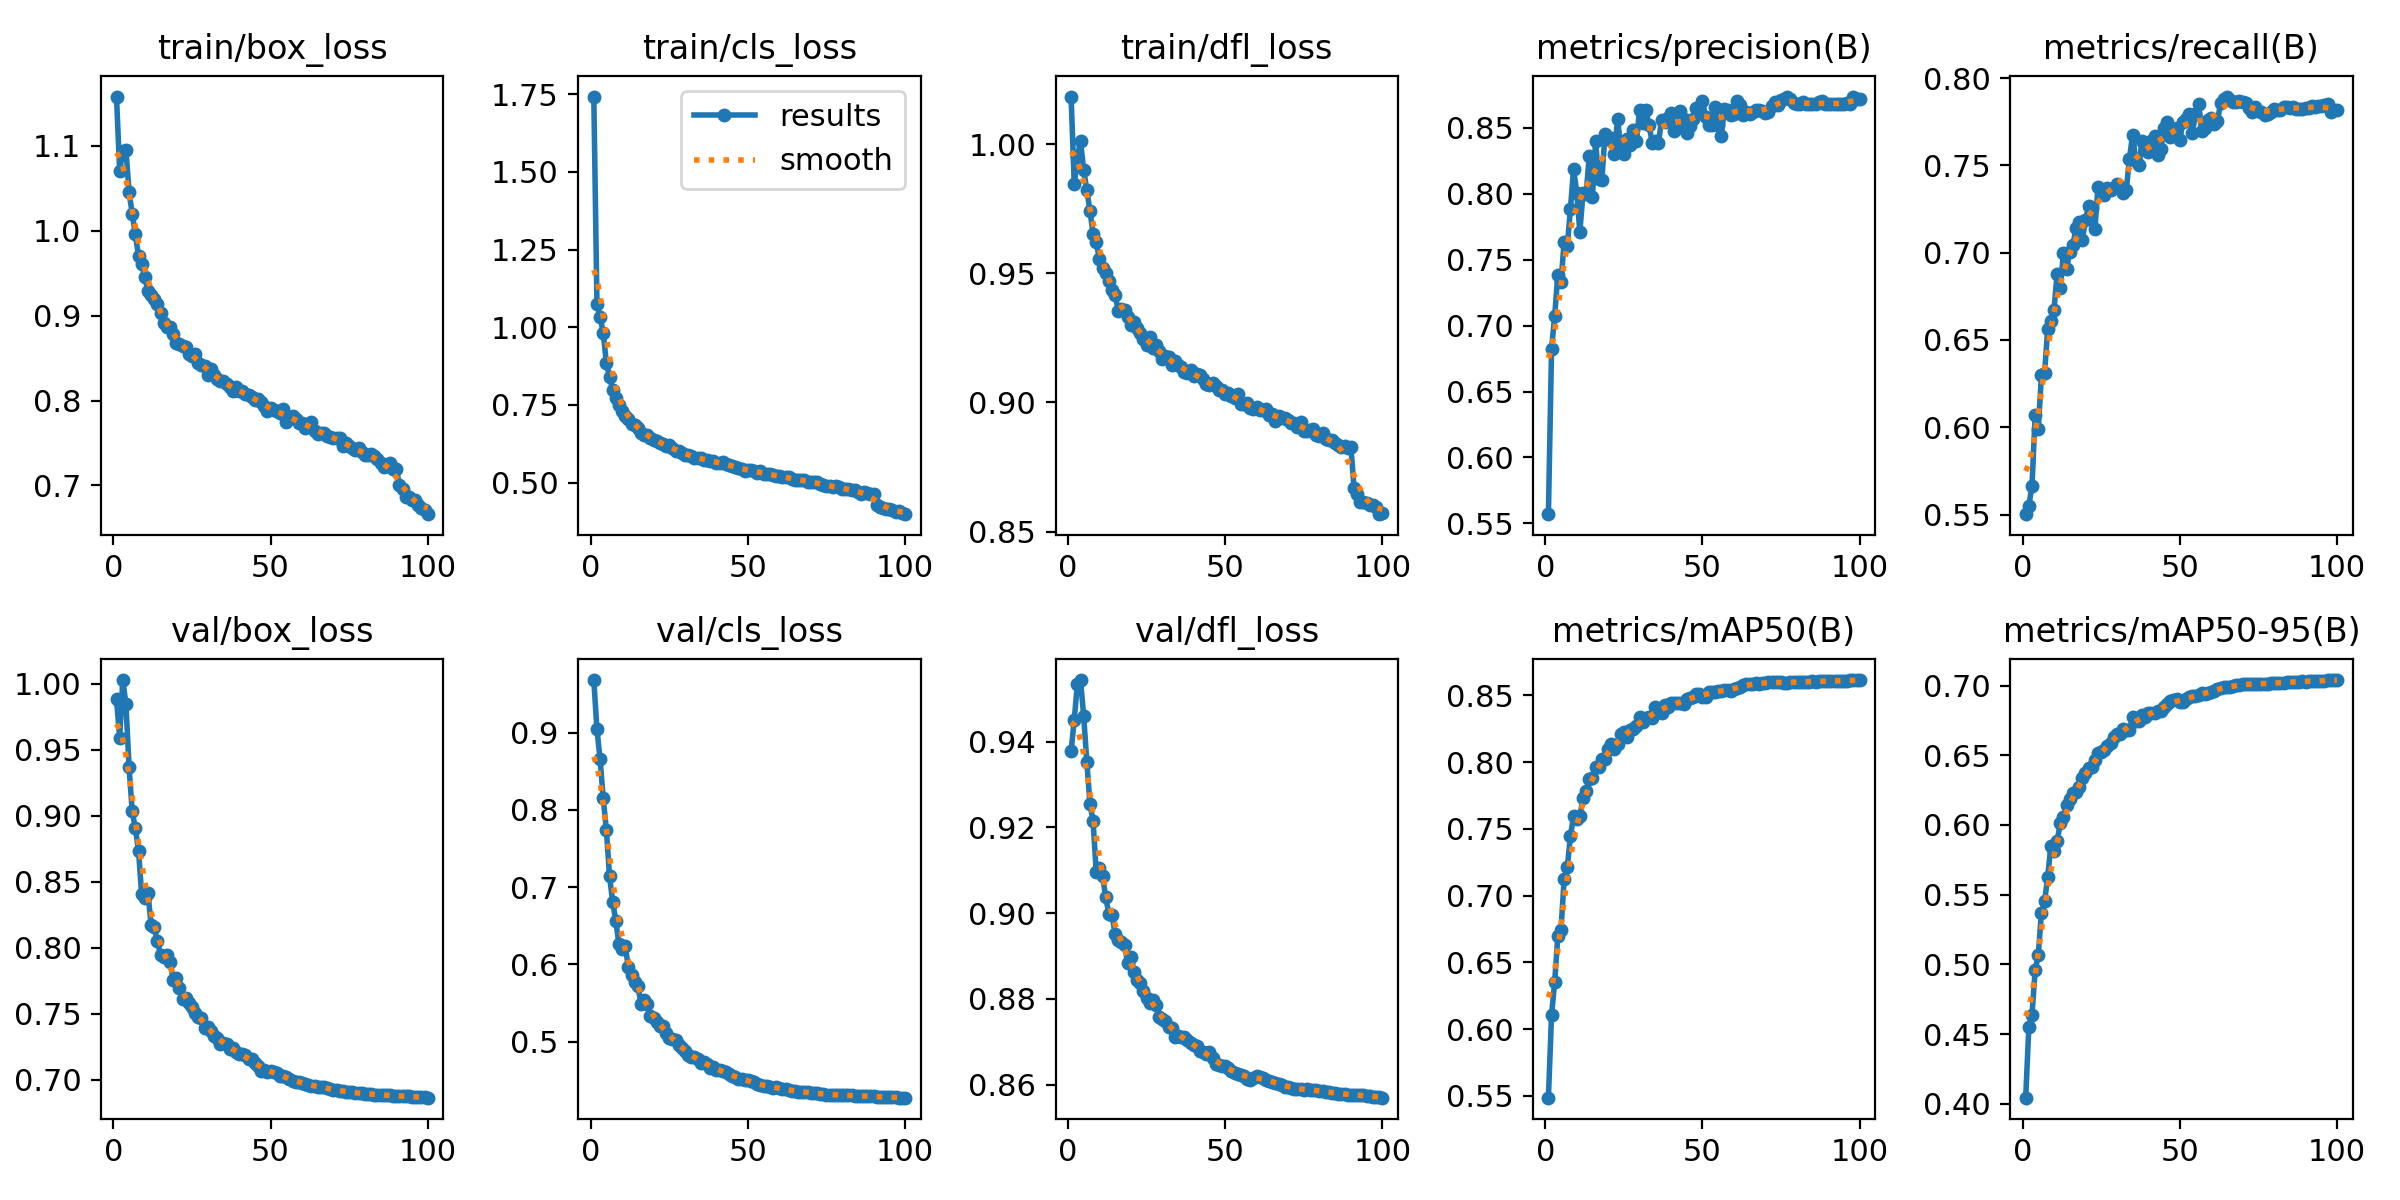
\includegraphics[width=0.9\linewidth]{Figures/results.png}
        \caption{Đồ thị Loss và mAP - Model 1}
    \end{figure}

    \framebreak

    \textbf{Kết quả chi tiết theo từng lớp:}
    \begin{table}
        \centering
        \begin{tabular}{|l|c|c|c|}
            \hline
            \textbf{Lớp} & \textbf{mAP@50} & \textbf{Precision} & \textbf{Recall} \\
            \hline
            Ô tô & \textbf{0.922} & 0.91 & 0.85 \\
            \hline
            Xe buýt & 0.897 & 0.88 & 0.80 \\
            \hline
            Xe máy & 0.872 & 0.85 & 0.79 \\
            \hline
            Xe tải & 0.832 & 0.84 & 0.75 \\
            \hline
            Xe đạp & 0.782 & 0.78 & 0.72 \\
            \hline
        \end{tabular}
    \end{table}

    \framebreak

    \begin{figure}
        \centering
        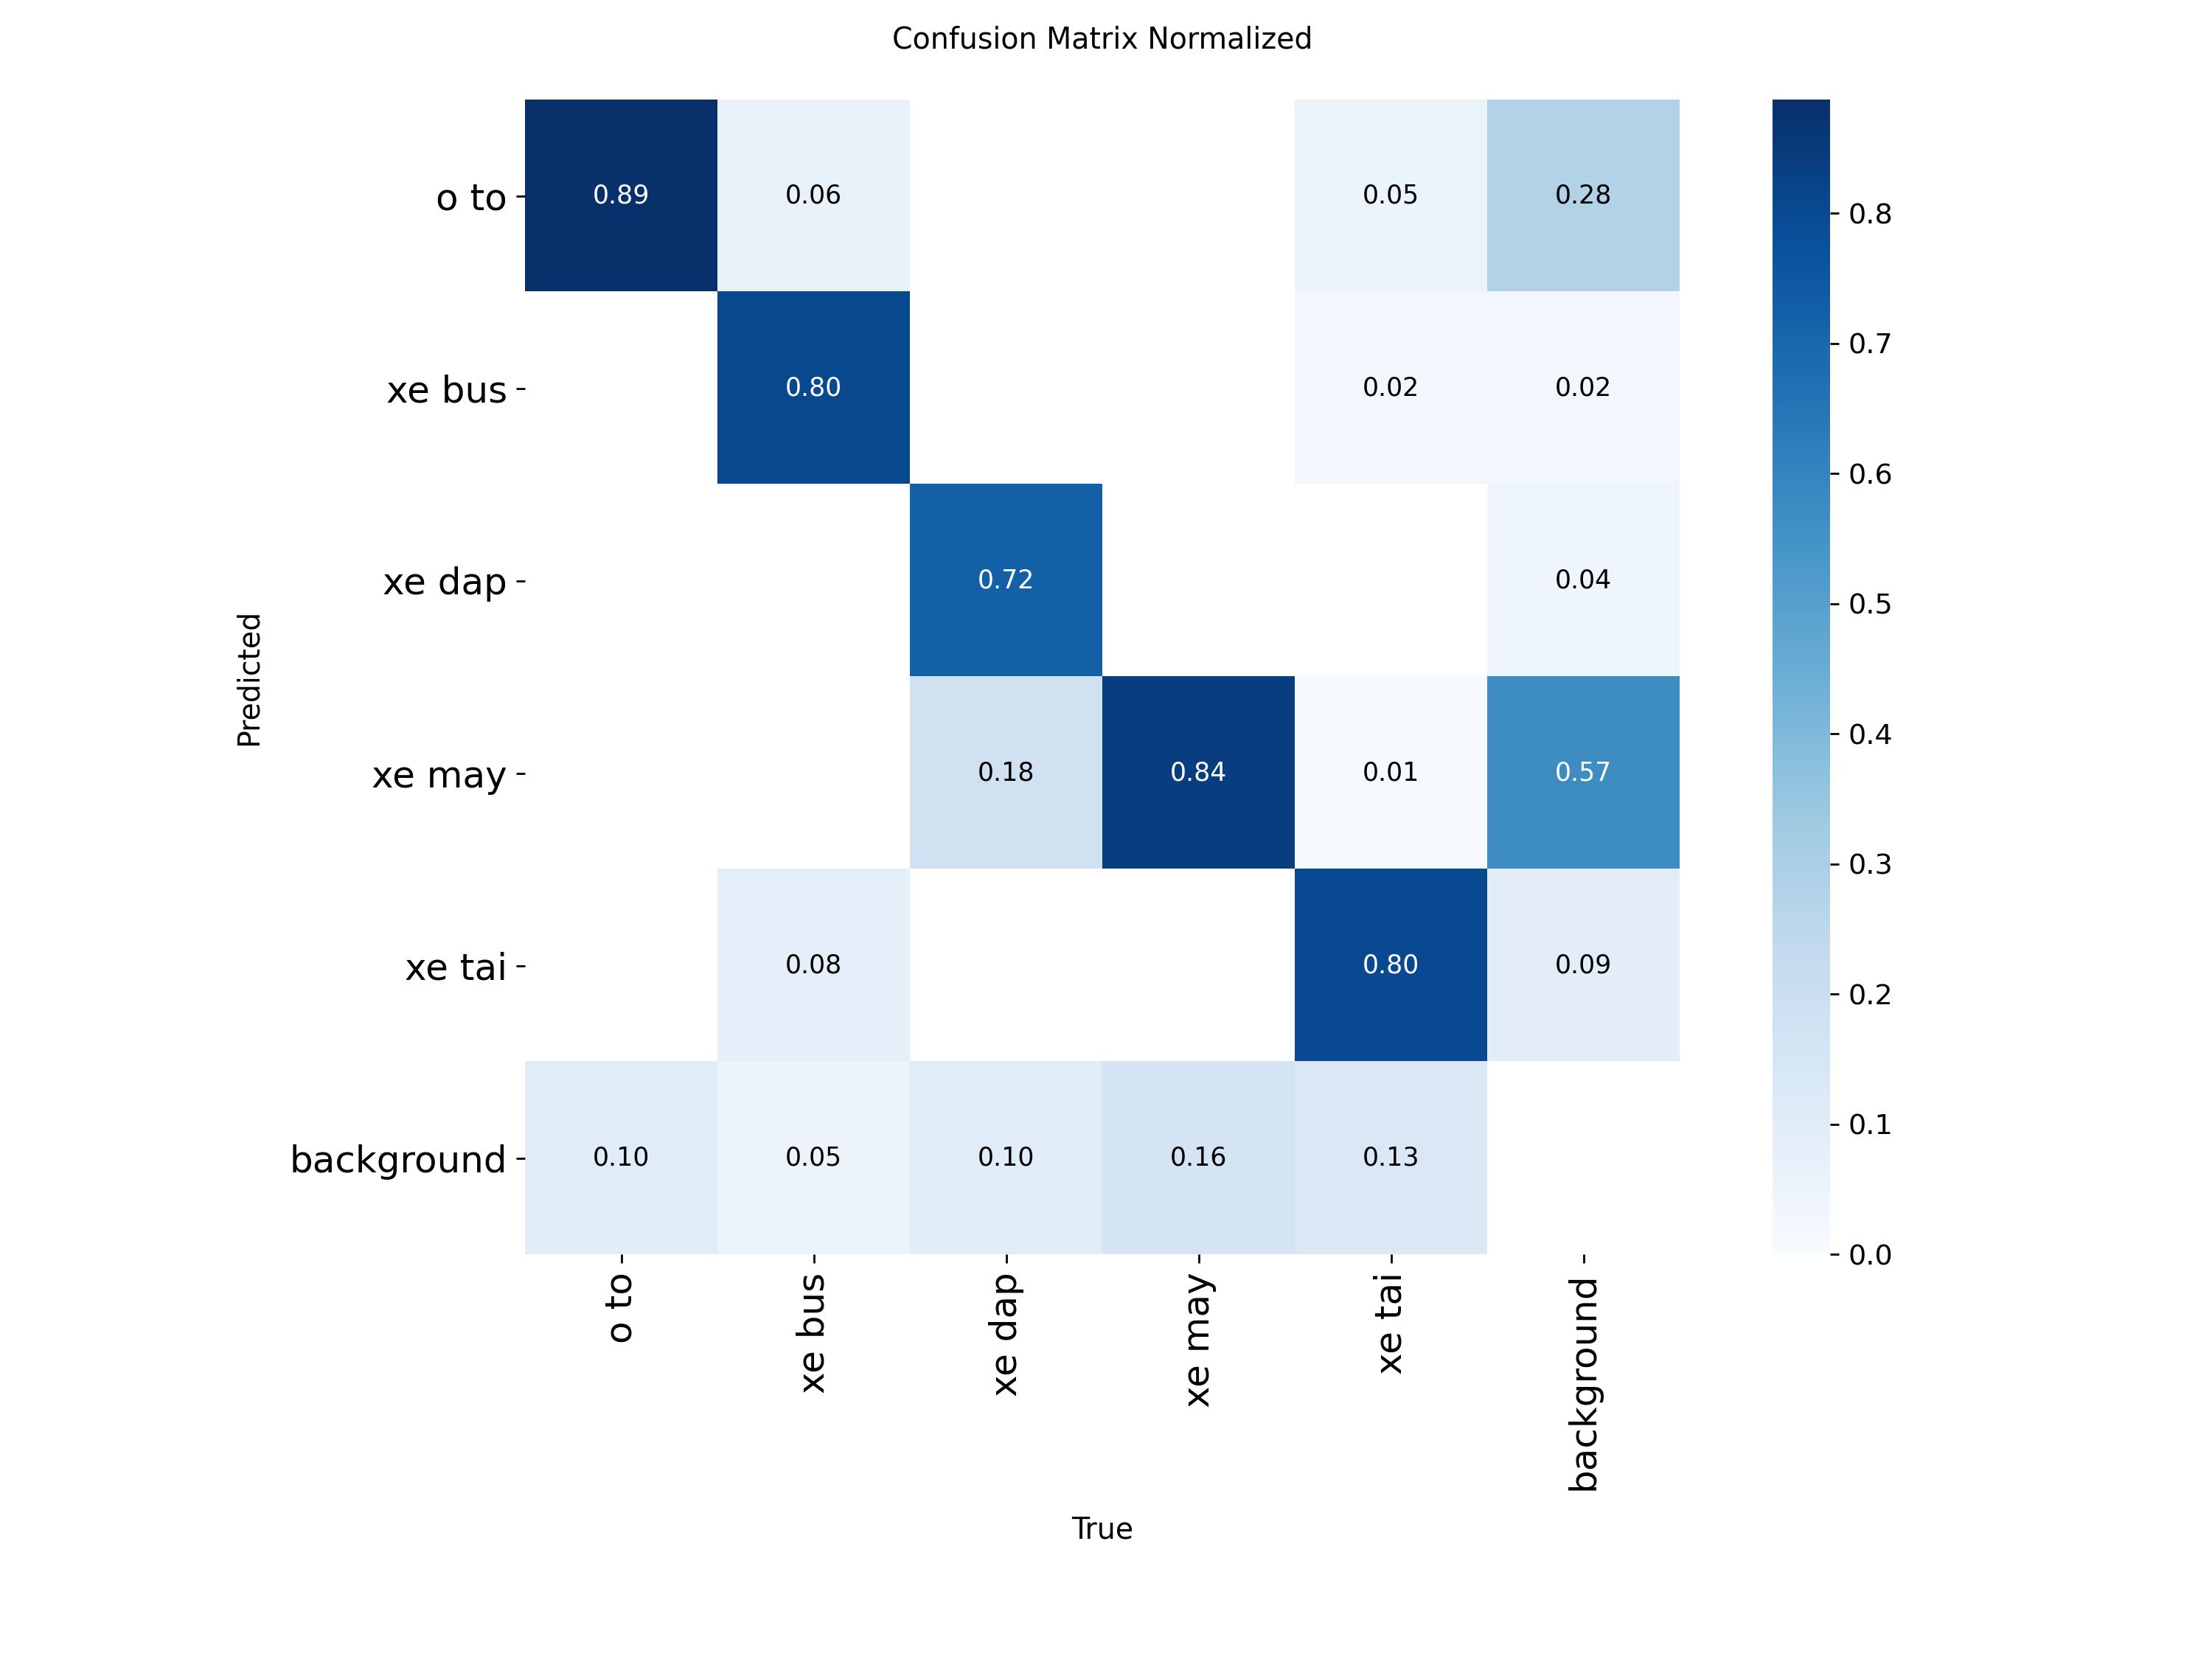
\includegraphics[width=0.65\linewidth]{Figures/confusion_matrix_normalized.png}
        \caption{Ma trận nhầm lẫn Model 1}
    \end{figure}

    \textbf{Nhận xét:} Nhầm lẫn chủ yếu giữa xe đạp và xe máy (18\%)
\end{frame}

%--- KẾT QUẢ MODEL 2 ---
\begin{frame}[allowframebreaks]{Kết quả Model 2: Phát hiện biển số}
    \begin{figure}
        \centering
        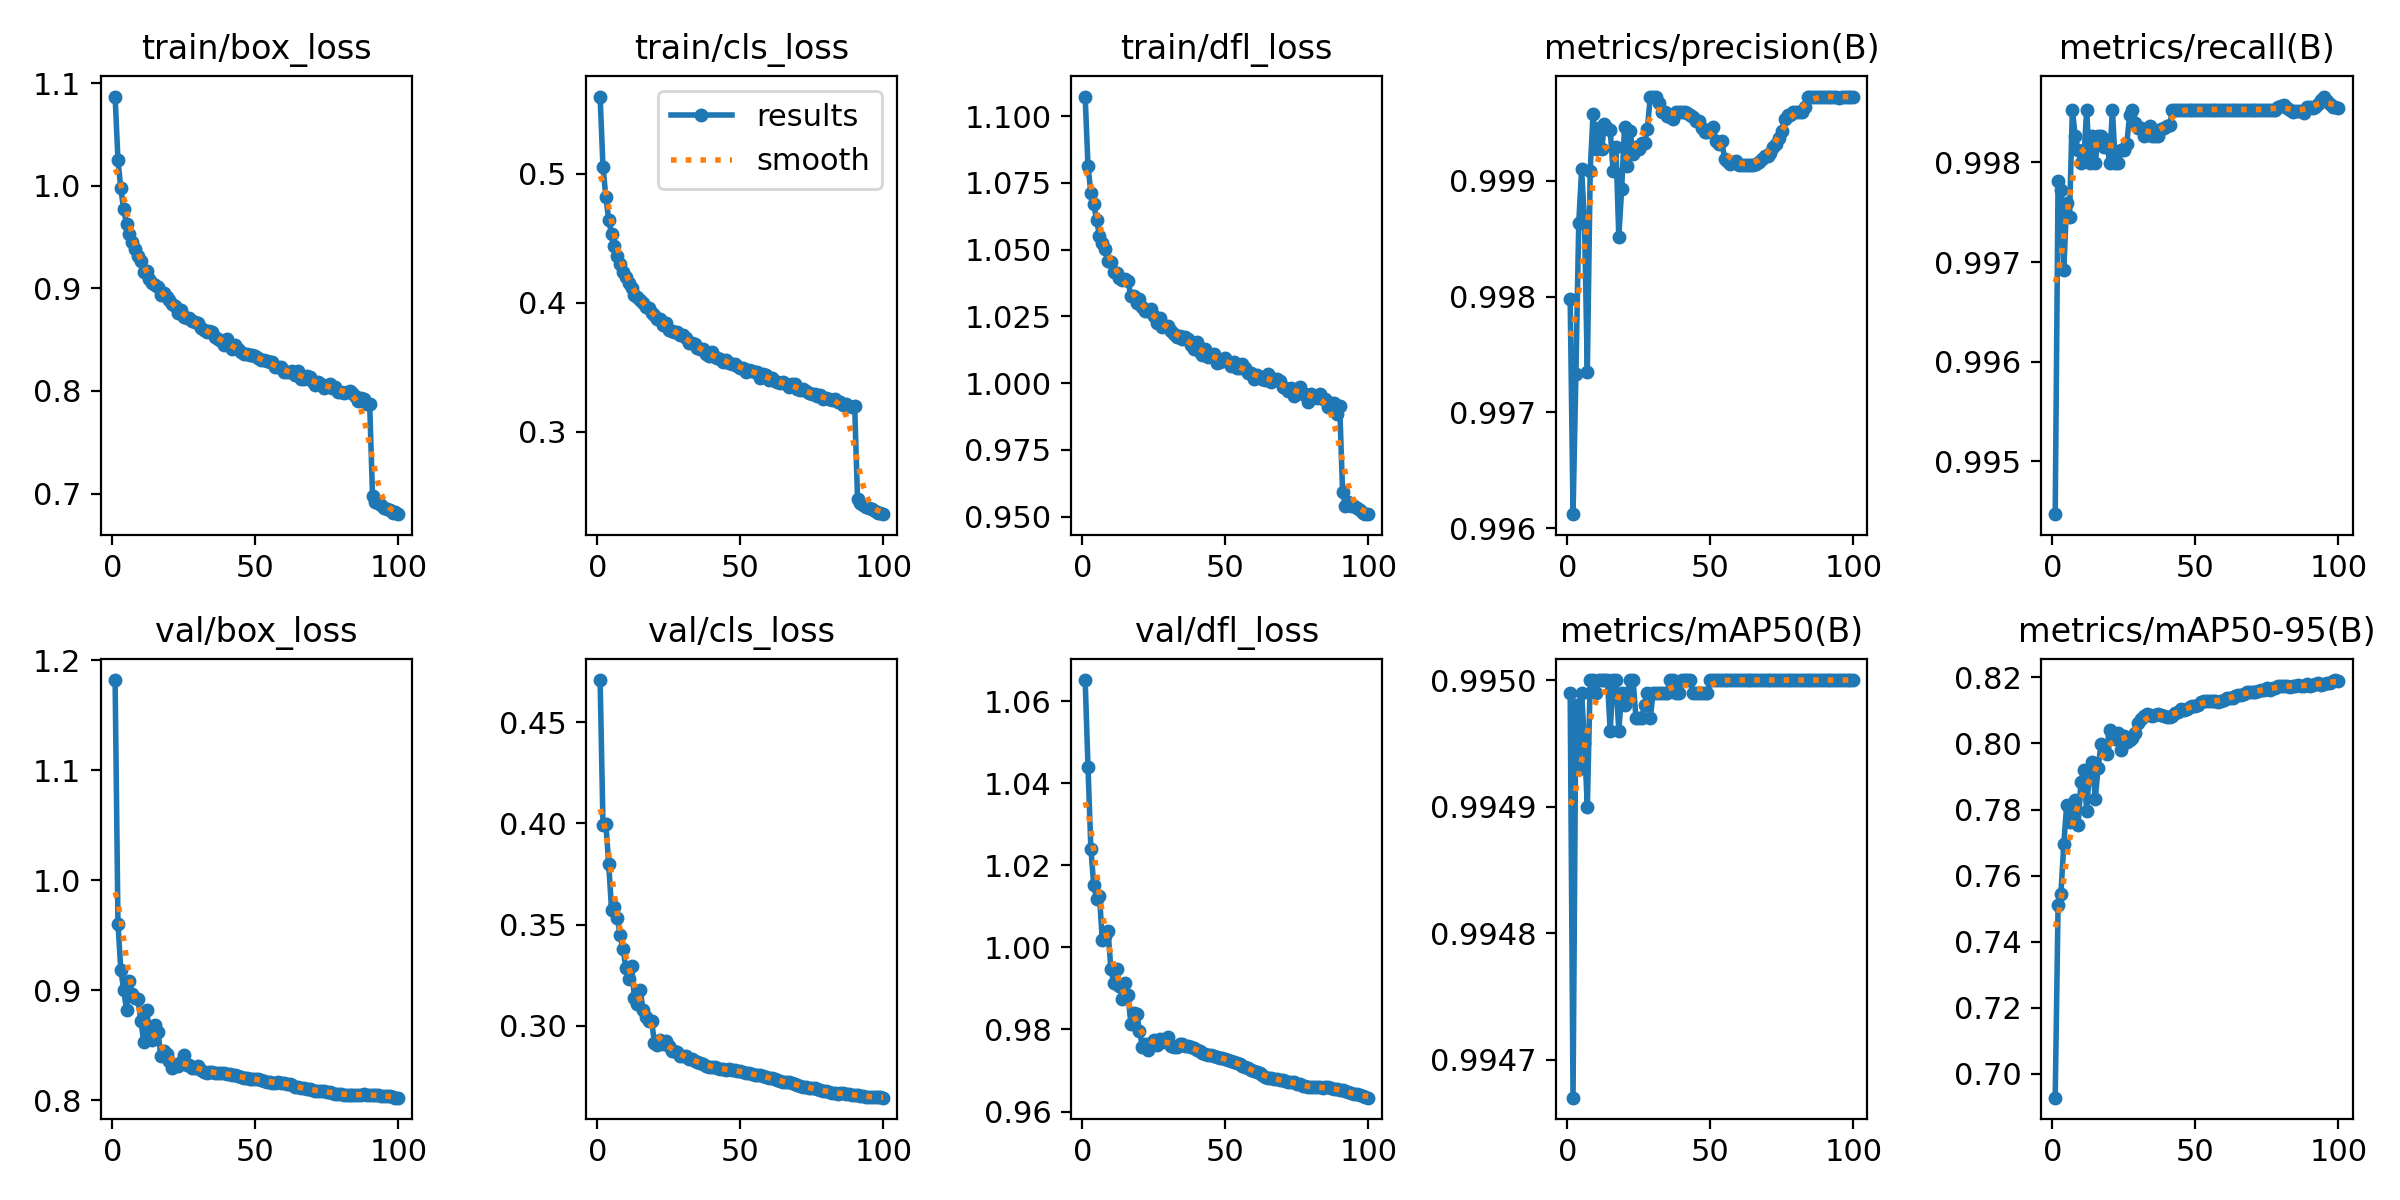
\includegraphics[width=0.9\linewidth]{Figures/plate_results.png}
        \caption{Đồ thị Loss và mAP - Model 2 (Plate Detection)}
    \end{figure}

    \framebreak

    \begin{alertblock}{Kết quả xuất sắc}
    \begin{itemize}
        \item \textbf{Precision:} 99.97\%
        \item \textbf{Recall:} 99.86\%
        \item \textbf{mAP@50:} 99.50\%
        \item \textbf{mAP@50-95:} 81.90\%
    \end{itemize}
    \end{alertblock}

    \textbf{Lý do đạt kết quả cao:}
    \begin{itemize}
        \item Bài toán phát hiện 1 lớp (single-class)
        \item Pretrained weights chất lượng
        \item Dataset VNLP đa dạng, được gán nhãn cẩn thận
    \end{itemize}

    \framebreak

    \begin{figure}
        \centering
        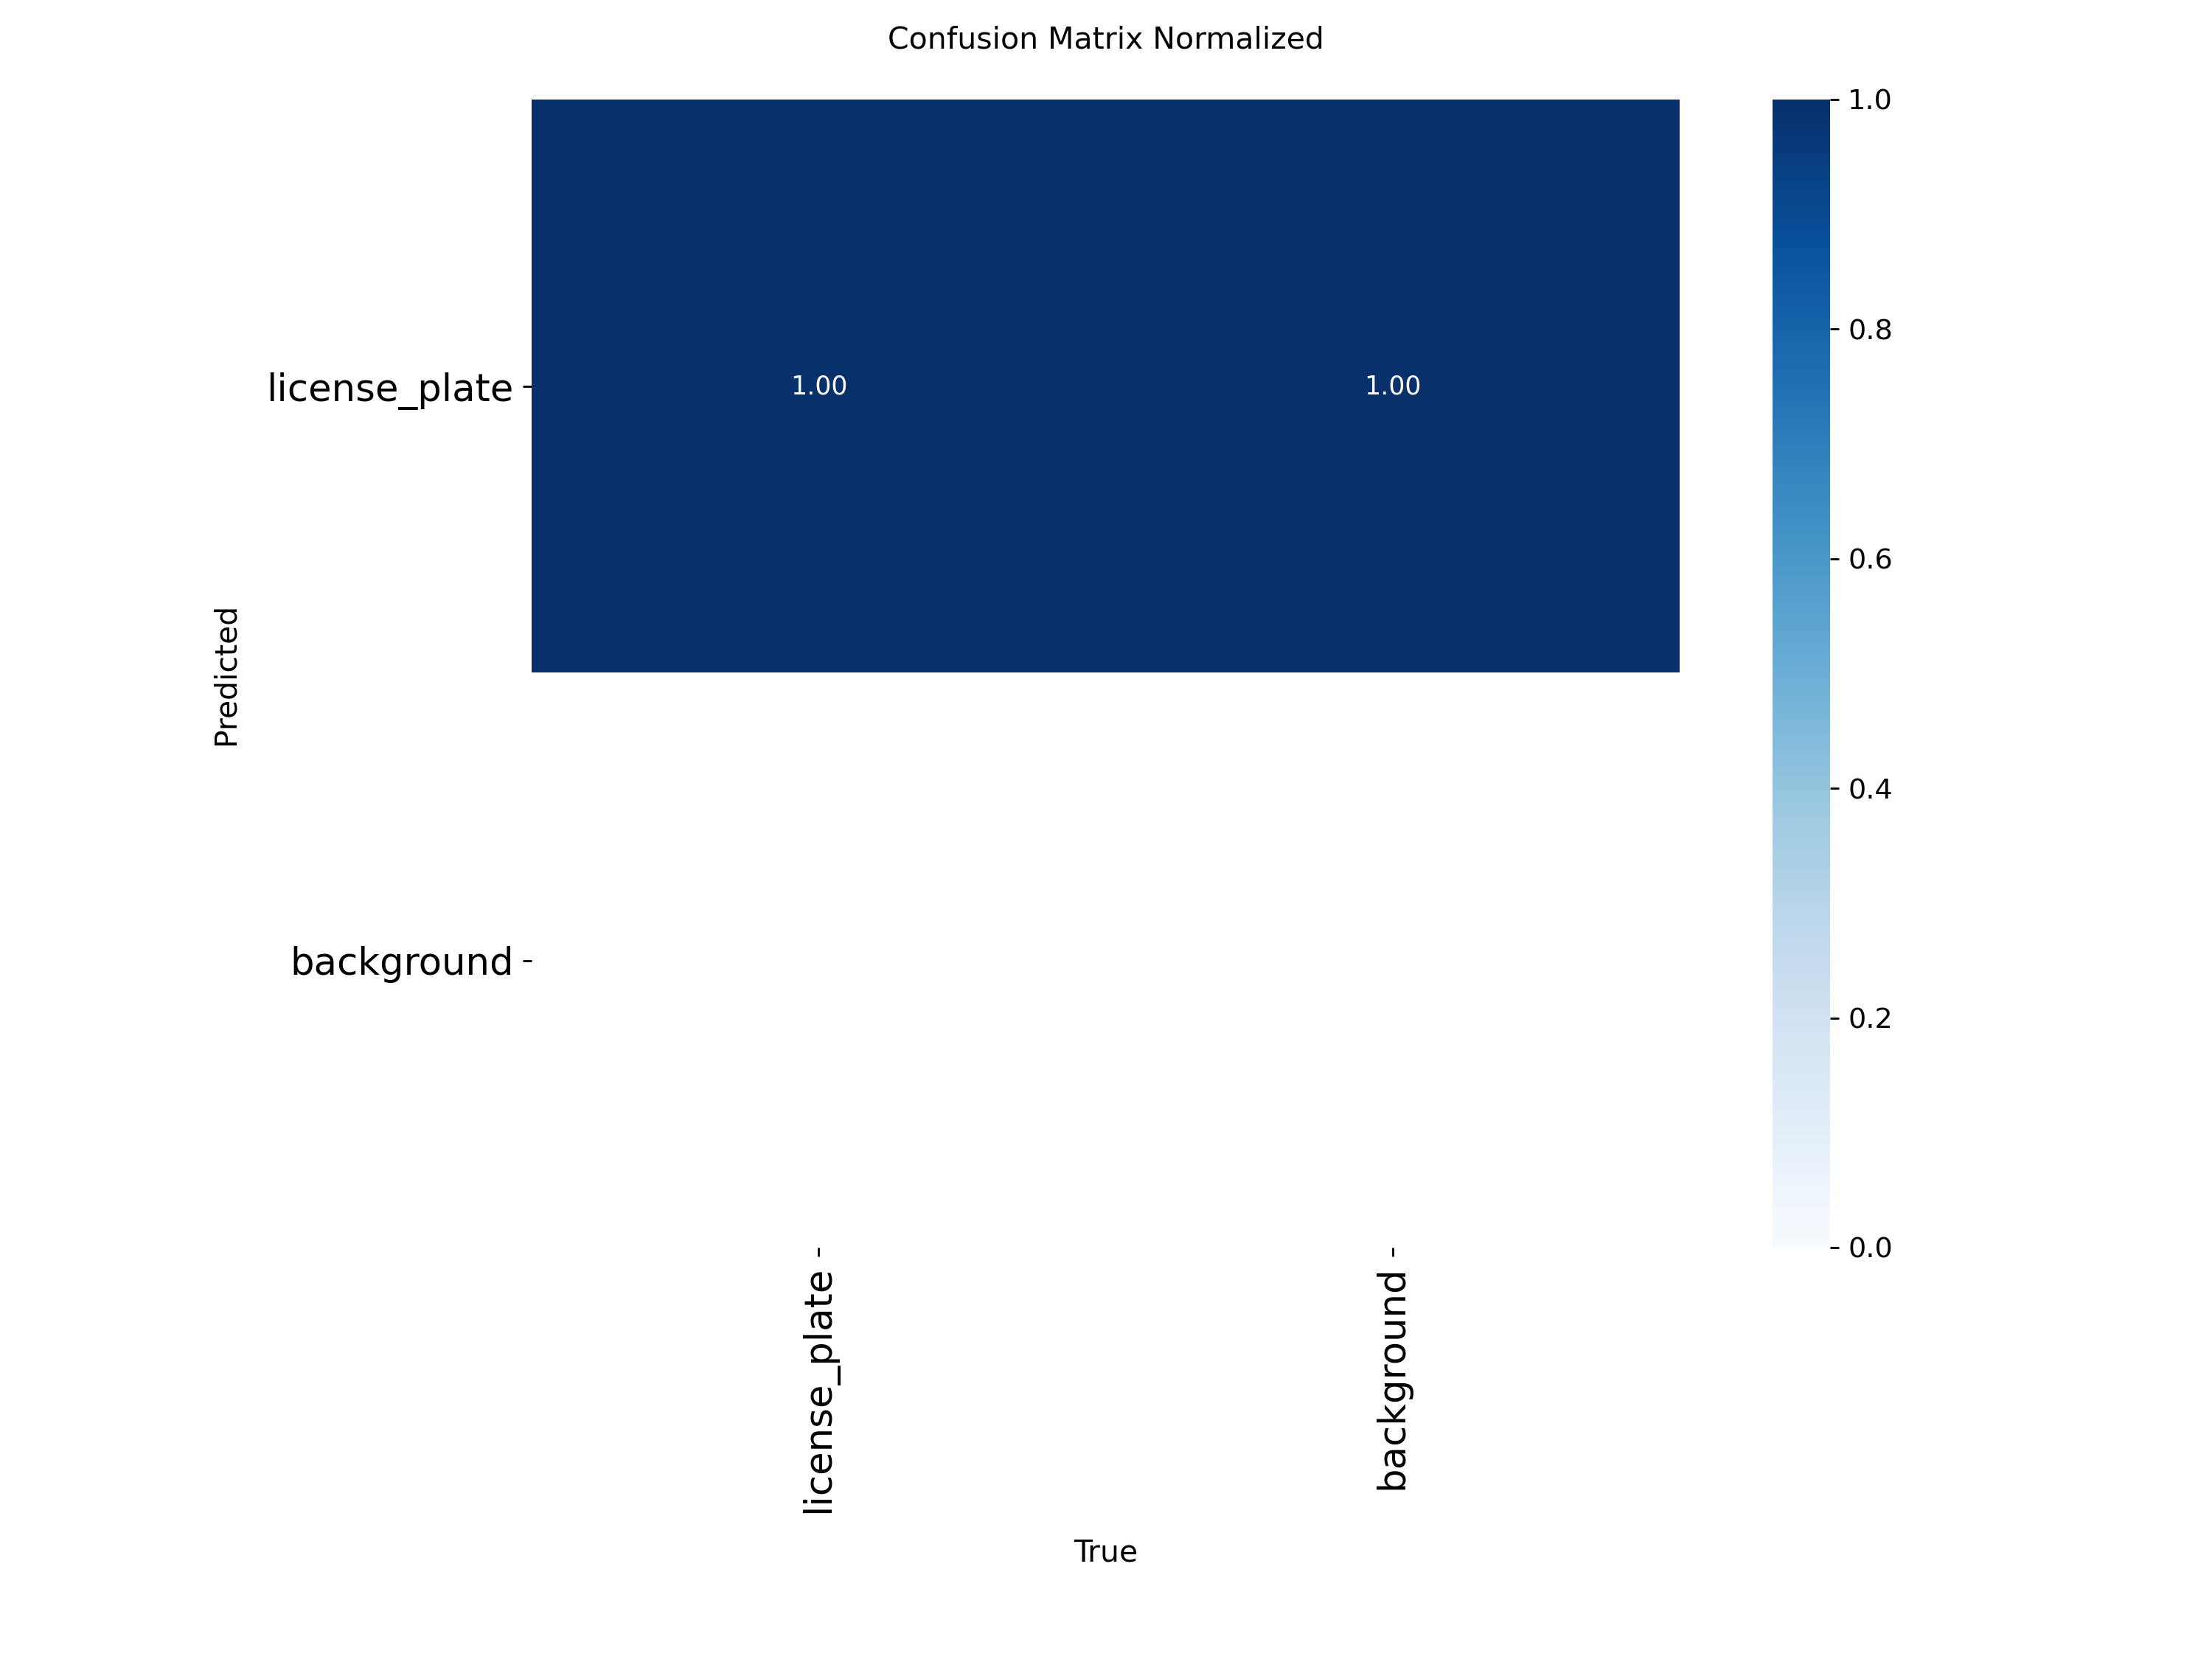
\includegraphics[width=0.55\linewidth]{Figures/plate_confusion_matrix.png}
        \caption{Ma trận nhầm lẫn Model 2 - Gần như hoàn hảo}
    \end{figure}
\end{frame}

%--- KẾT QUẢ MODEL TÍCH HỢP ---
\begin{frame}[allowframebreaks]{Kết quả Mô hình tích hợp 6 lớp}
    \begin{figure}
        \centering
        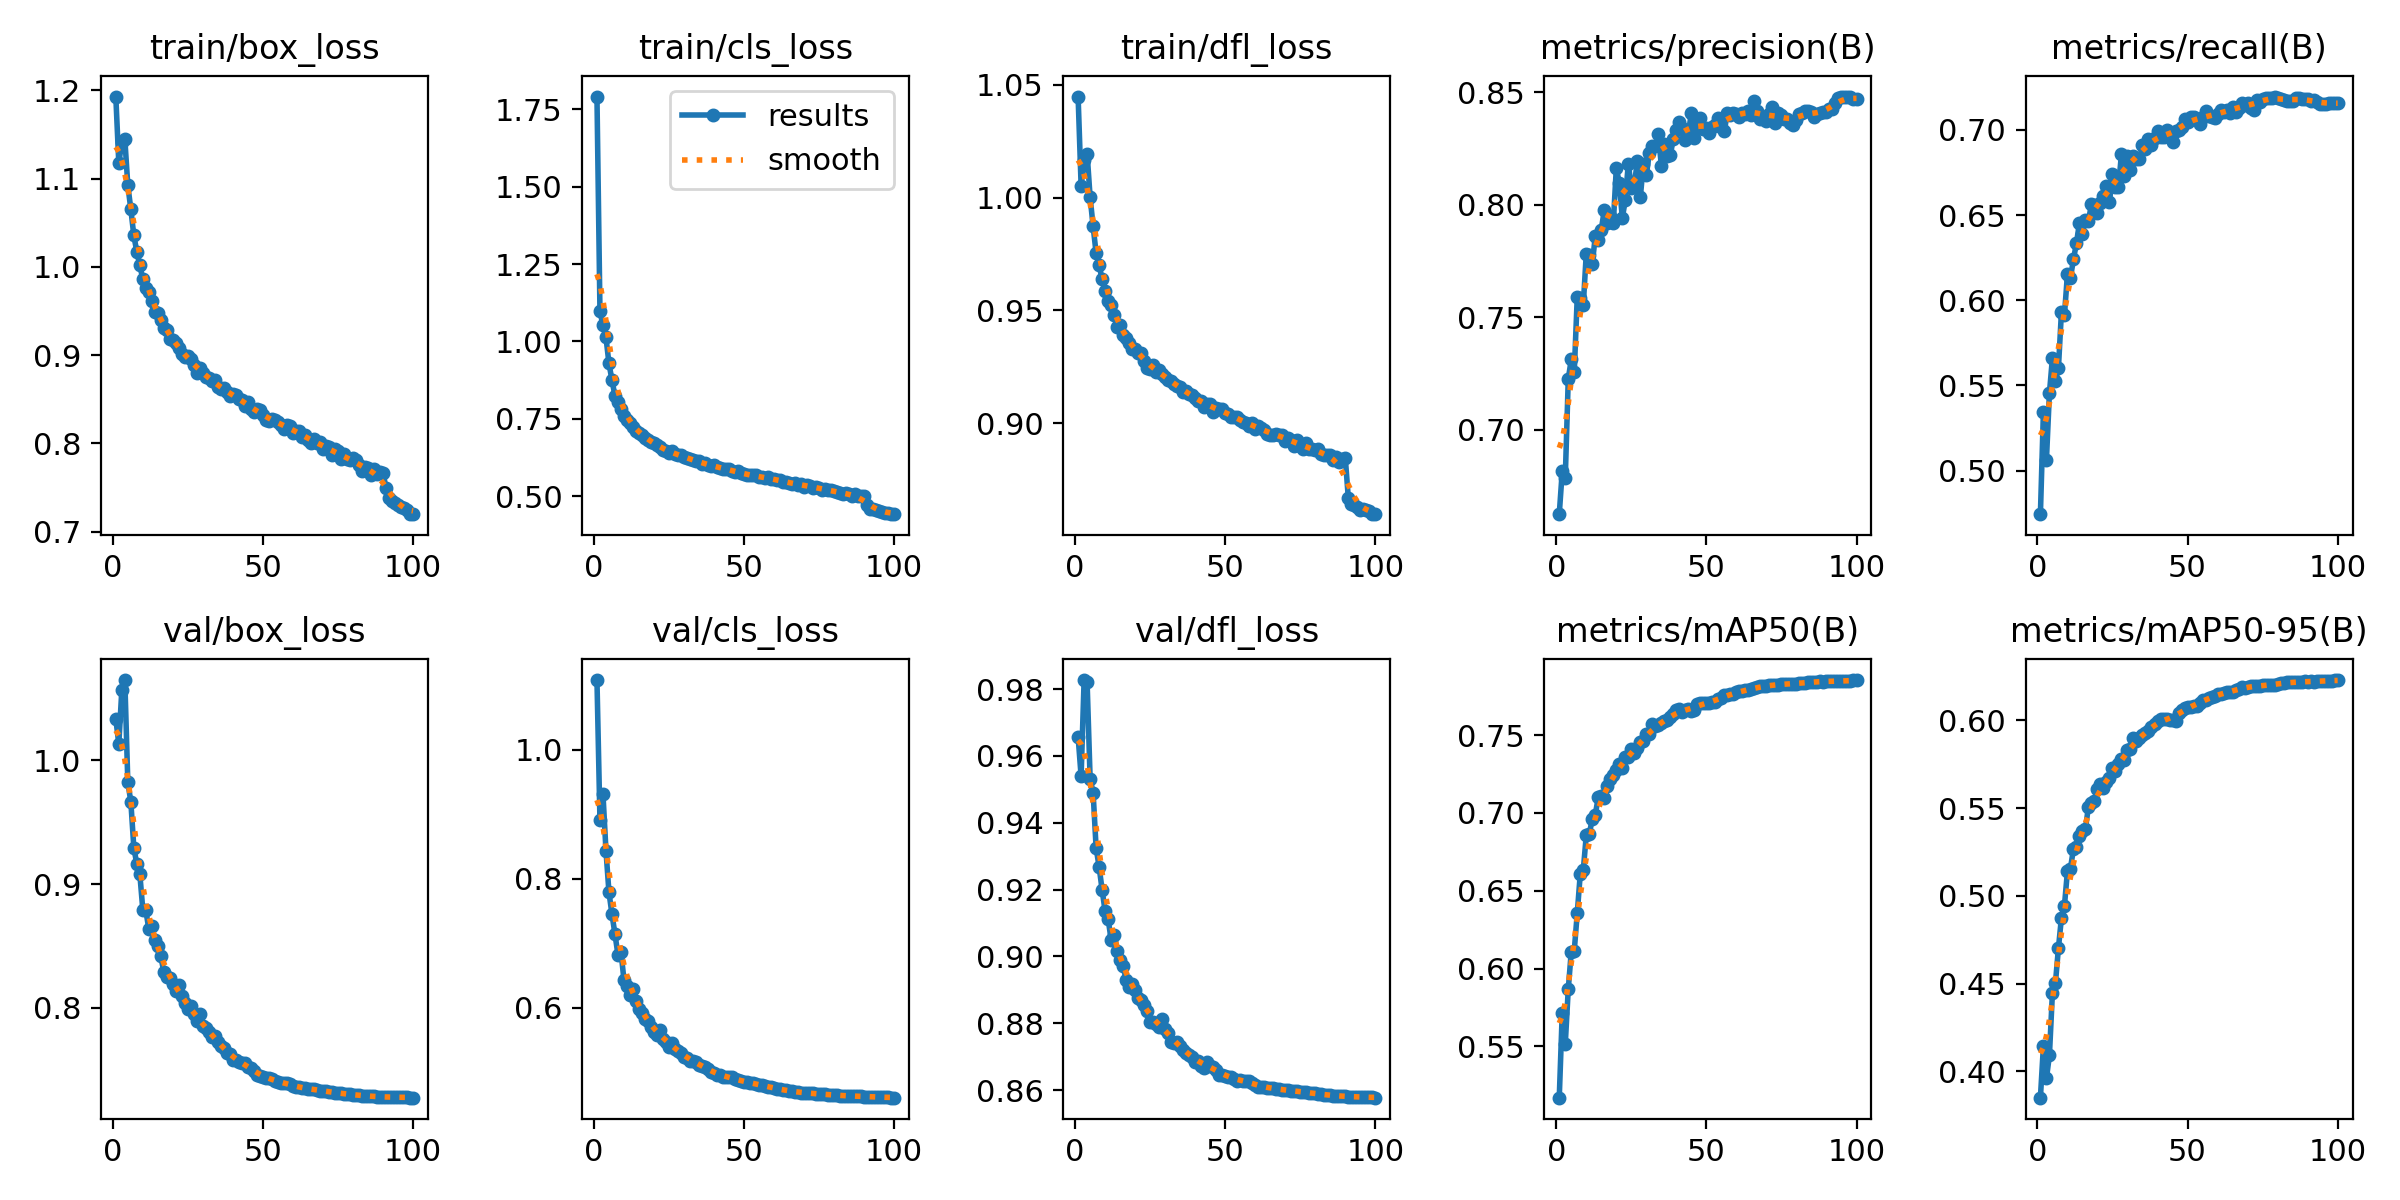
\includegraphics[width=0.9\linewidth]{Figures/multiclass_results.png}
        \caption{Đồ thị Loss và mAP - Mô hình tích hợp}
    \end{figure}

    \framebreak

    \textbf{Kết quả theo từng lớp:}
    \begin{table}
        \centering
        \begin{tabular}{|l|c|c|c|}
            \hline
            \textbf{Lớp} & \textbf{mAP@50} & \textbf{Precision} & \textbf{Recall} \\
            \hline
            Ô tô & 0.89 & 0.88 & 0.82 \\
            \hline
            Xe buýt & 0.86 & 0.85 & 0.78 \\
            \hline
            Xe máy & 0.84 & 0.83 & 0.76 \\
            \hline
            Xe tải & 0.81 & 0.82 & 0.73 \\
            \hline
            Xe đạp & 0.72 & 0.75 & 0.65 \\
            \hline
            \textbf{Biển số} & \textbf{0.59} & 0.72 & 0.56 \\
            \hline
        \end{tabular}
    \end{table}

    \textbf{Hạn chế:} Lớp biển số có mAP thấp (0.59) do class imbalance và kích thước nhỏ
\end{frame}

%--- KẾT QUẢ INFERENCE PIPELINE 2 ---
\begin{frame}[allowframebreaks]{Kết quả Inference Pipeline 2 (One-Stage)}
    \begin{figure}
        \centering
        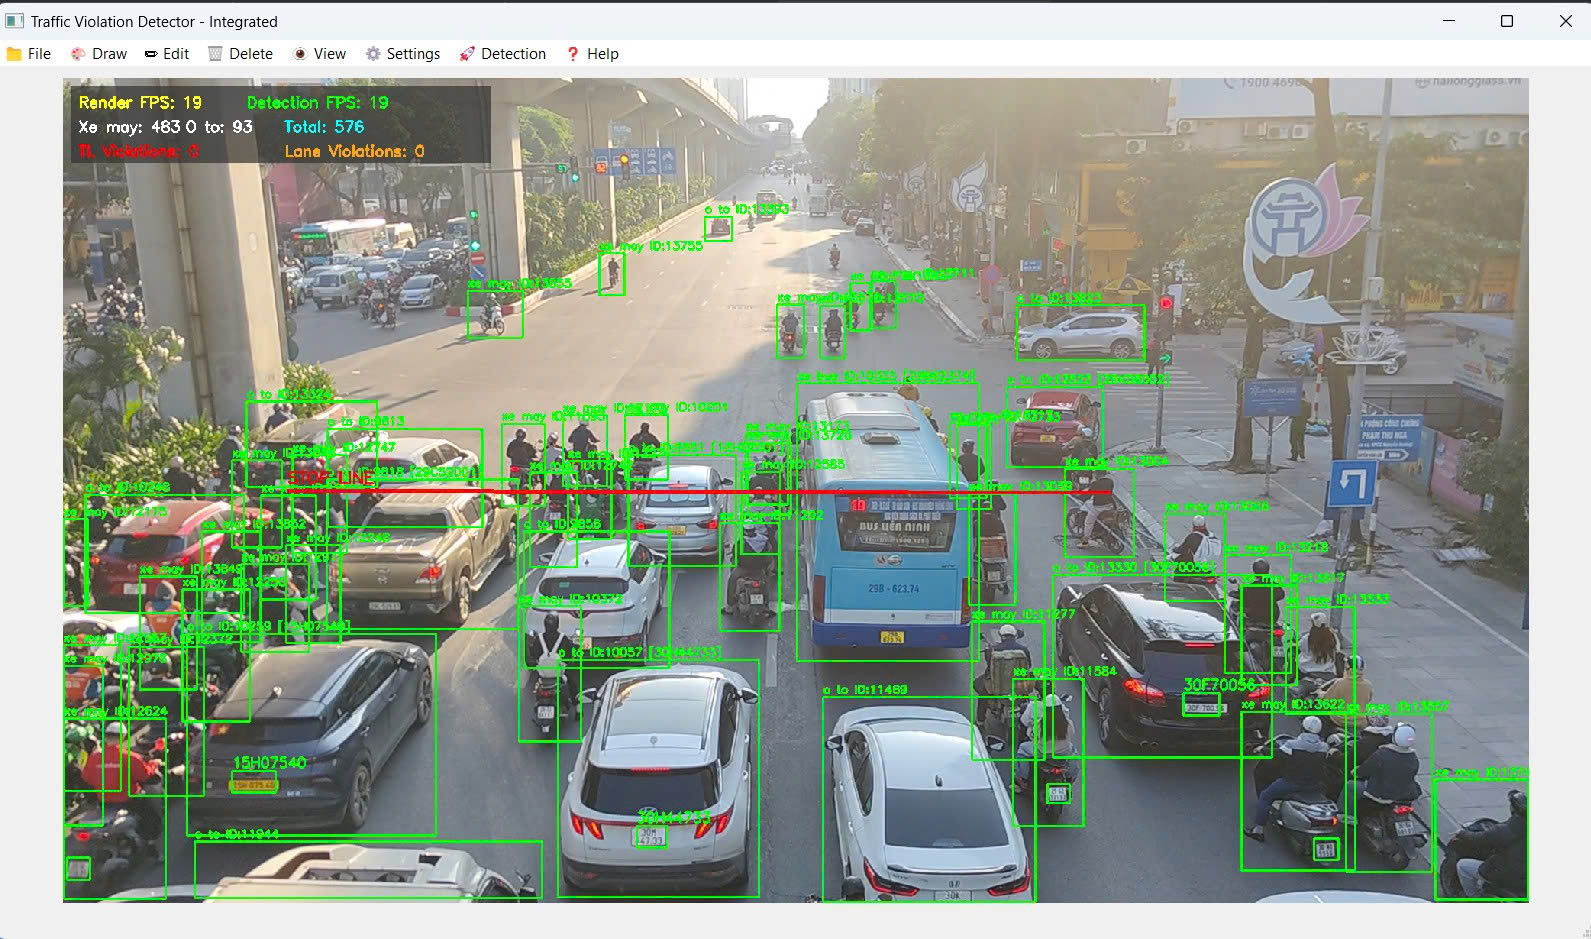
\includegraphics[width=0.85\linewidth]{Figures/ppthucnghiem2.jpg}
        \caption{Pipeline 2: Phát hiện đồng thời xe và biển số (1 model)}
    \end{figure}

    \framebreak

    \textbf{Ưu điểm quan sát được:}
    \begin{itemize}
        \item Phát hiện tốt các loại phương tiện với bbox chính xác
        \item Biển số được phát hiện khi có kích thước đủ lớn
        \item Mapping plate$\rightarrow$xe tự động qua containment check (95\% thành công)
    \end{itemize}

    \textbf{Hạn chế:}
    \begin{itemize}
        \item Biển số nhỏ/xa có thể bị bỏ sót
        \item Trade-off: Tốc độ nhanh nhưng mAP plate giảm
    \end{itemize}
\end{frame}

%--- SO SÁNH PIPELINE ---
\begin{frame}{So sánh hiệu năng hai Pipeline ALPR}
    \begin{table}
        \centering
        \small
        \begin{tabular}{|l|c|c|}
            \hline
            \textbf{Tiêu chí} & \textbf{Pipeline 1} & \textbf{Pipeline 2} \\
            & \textbf{(Two-Stage)} & \textbf{(One-Stage)} \\
            \hline
            FPS trung bình & 5--10 FPS & 15--20 FPS \\
            \hline
            mAP@50 (Plate) & \textbf{99.5\%} & 59\% \\
            \hline
            Số model cần load & 2 & 1 \\
            \hline
            GPU Memory & ~2.5GB & ~1.2GB \\
            \hline
            Phát hiện biển nhỏ & \textbf{Tốt} & Trung bình \\
            \hline
            Tài nguyên tiêu thụ & Cao & Thấp \\
            \hline
        \end{tabular}
        \caption{So sánh hai phương pháp ALPR (theo báo cáo)}
    \end{table}
\end{frame}

\begin{frame}{Khuyến nghị sử dụng}
    \begin{block}{Pipeline 1 (Two-Stage) - Ưu tiên độ chính xác}
    \begin{itemize}
        \item Yêu cầu độ chính xác cao cho biển số
        \item Camera có độ phân giải tốt
        \item Biển số nhỏ hoặc ở xa
    \end{itemize}
    \end{block}

    \begin{block}{Pipeline 2 (One-Stage) - Ưu tiên tốc độ}
    \begin{itemize}
        \item Yêu cầu xử lý real-time
        \item Tài nguyên phần cứng hạn chế
        \item Biển số đủ lớn trong khung hình
    \end{itemize}
    \end{block}
\end{frame}

%--- ĐÁNH GIÁ BYTETRACK ---
\begin{frame}{Đánh giá ByteTrack Tracking}
    \begin{block}{Kết quả thực tế}
    \begin{itemize}
        \item \textbf{ID Switch Rate:} < 5\% trên video thử nghiệm
        \item \textbf{Overhead:} ~2ms mỗi frame
        \item \textbf{Tính năng:} Kalman Filter + Hungarian Matching
    \end{itemize}
    \end{block}

    \begin{block}{Quan sát thực tế}
    \begin{itemize}
        \item \textbf{Hoạt động tốt:} Xe di chuyển bình thường, mật độ cao
        \item \textbf{ID switch xảy ra khi:}
        \begin{itemize}
            \item Xe bị che khuất > 2 giây
            \item Thay đổi tốc độ đột ngột
            \item Xe quá gần nhau (occlusion)
        \end{itemize}
    \end{itemize}
    \end{block}

    \textit{Cải thiện tiềm năng: Kết hợp Re-ID features}
\end{frame}

%--- ĐÁNH GIÁ OCR ---
\begin{frame}{Đánh giá OCR (PaddleOCR)}
    \begin{block}{Hiệu quả Format Validation}
    \begin{itemize}
        \item Loại bỏ kết quả nhiễu ngay từ đầu
        \item Chỉ hiển thị biển số đúng format VN
        \item Tận dụng tracking để retry tự động
    \end{itemize}
    \end{block}

    \textbf{Các trường hợp khó:}
    \begin{enumerate}
        \item Biển số bẩn/mờ: CLAHE giúp cải thiện nhưng hạn chế
        \item Góc nghiêng lớn: Perspective distortion giảm độ chính xác
        \item Ban đêm: Phản sáng từ đèn flash làm mất chi tiết
        \item Biển nhỏ/xa: Độ phân giải thấp
    \end{enumerate}
\end{frame}

%----------------------------------------------------------------------------------------
%   PHẦN 5: DEMO VÀ KẾT LUẬN
%----------------------------------------------------------------------------------------
\section{Demo và Kết luận}

%--- GIAO DIỆN HỆ THỐNG ---
\begin{frame}{Giao diện hệ thống}
    \begin{columns}
        \column{0.5\textwidth}
        \textbf{Tính năng chính:}
        \begin{itemize}
            \item Chọn video/camera đầu vào
            \item Cấu hình ROI (Stopline, Lanes)
            \item Chọn Pipeline ALPR
            \item Hiển thị real-time
            \item Xuất báo cáo vi phạm
        \end{itemize}

        \column{0.5\textwidth}
        \textbf{Thành phần UI:}
        \begin{itemize}
            \item Control Panel (bên trái)
            \item Video Display (giữa)
            \item Info Panel (bên phải)
            \item Status Bar (dưới)
        \end{itemize}
    \end{columns}

    \vspace{0.5em}
    \textit{Framework: PyQt5 + OpenCV}
\end{frame}

%--- KẾT QUẢ INFERENCE ---
\begin{frame}[allowframebreaks]{Kết quả Inference thực tế}
    \begin{figure}
        \centering
        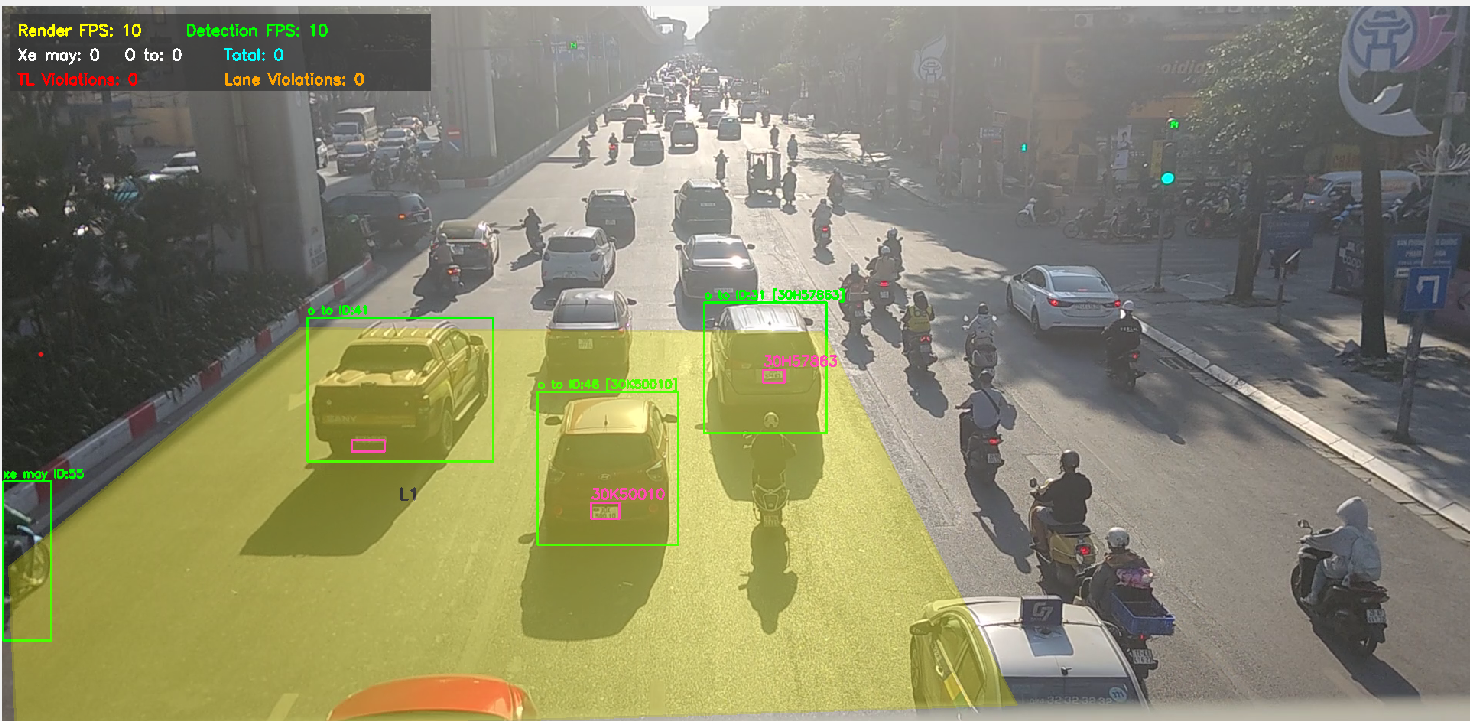
\includegraphics[width=0.85\linewidth]{Figures/plate_inference1.png}
        \caption{Pipeline 1: Phát hiện biển số chính xác}
    \end{figure}

    \framebreak

    \begin{figure}
        \centering
        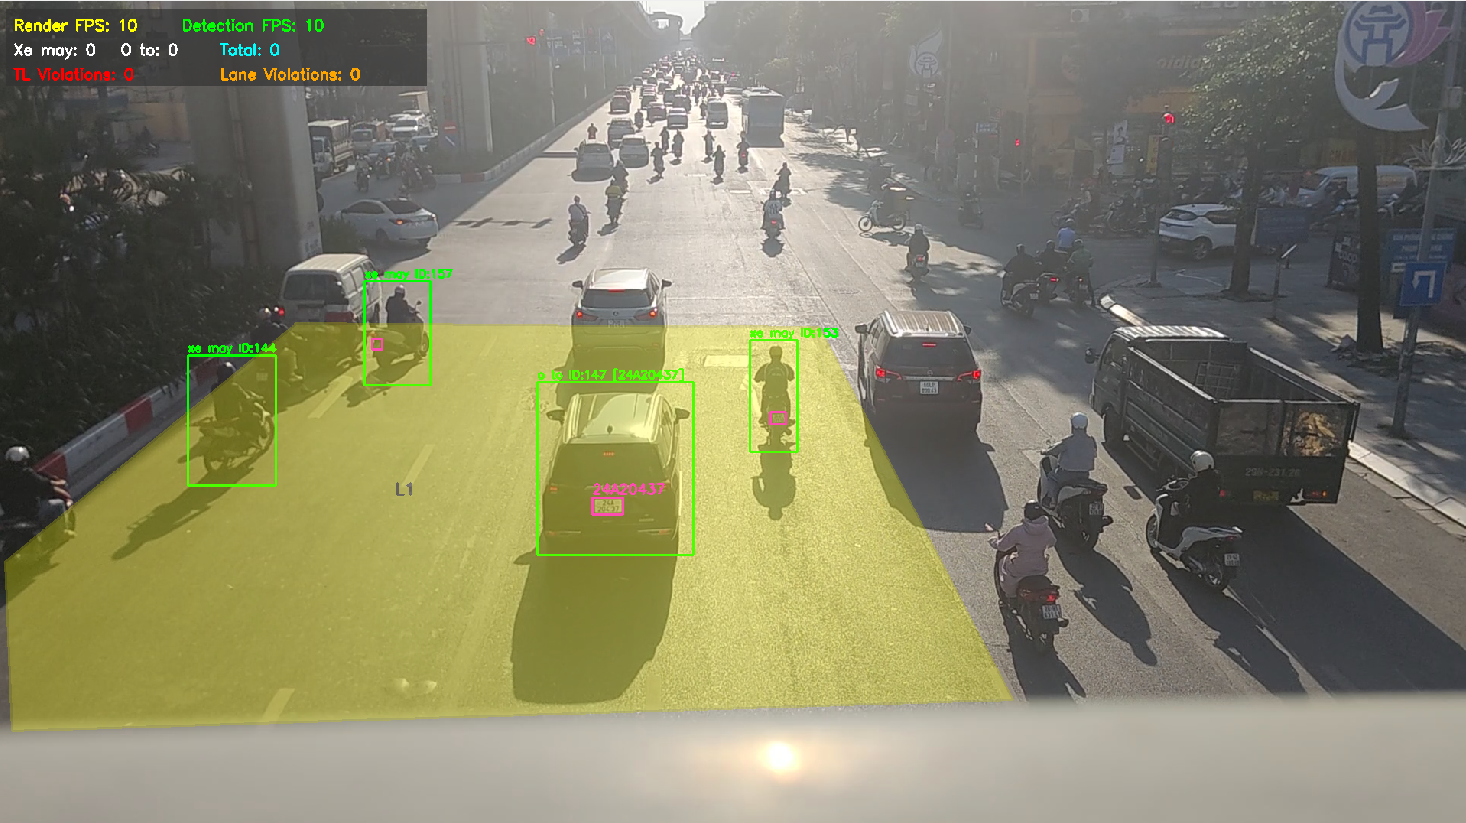
\includegraphics[width=0.85\linewidth]{Figures/plate_inference2.png}
        \caption{Pipeline 1: OCR nhận dạng biển số Việt Nam}
    \end{figure}

    \framebreak

    \begin{figure}
        \centering
        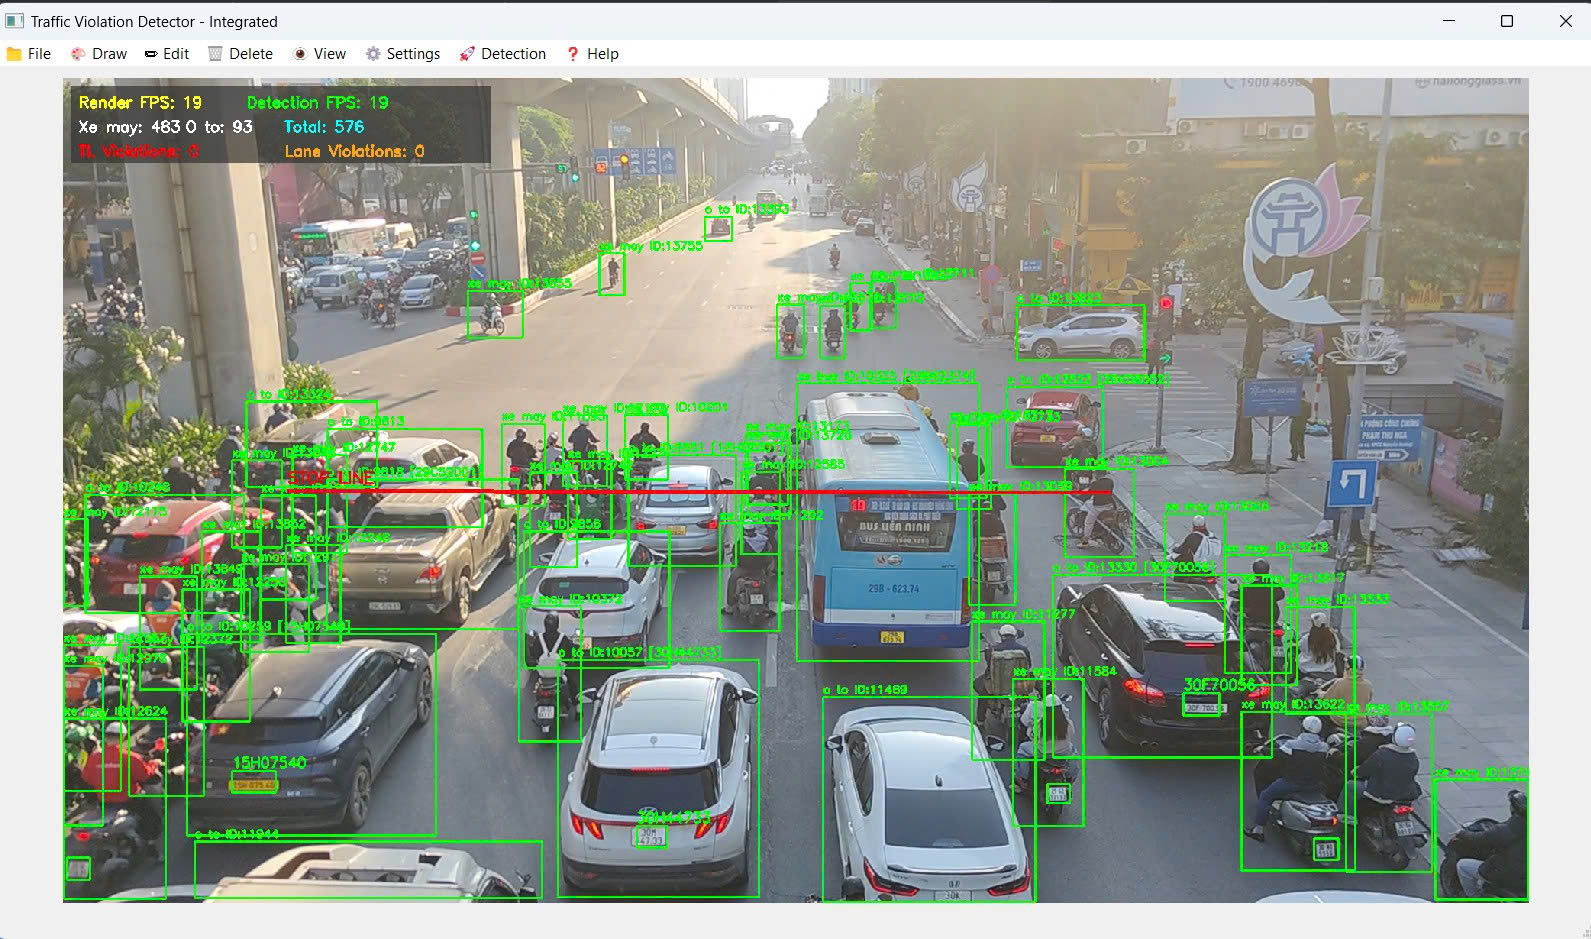
\includegraphics[width=0.85\linewidth]{Figures/ppthucnghiem2.jpg}
        \caption{Pipeline 2: Phát hiện đồng thời xe và biển số}
    \end{figure}
\end{frame}

%--- PHÁT HIỆN VI PHẠM ---
\begin{frame}[allowframebreaks]{Kết quả phát hiện vi phạm}
    \begin{figure}
        \centering
        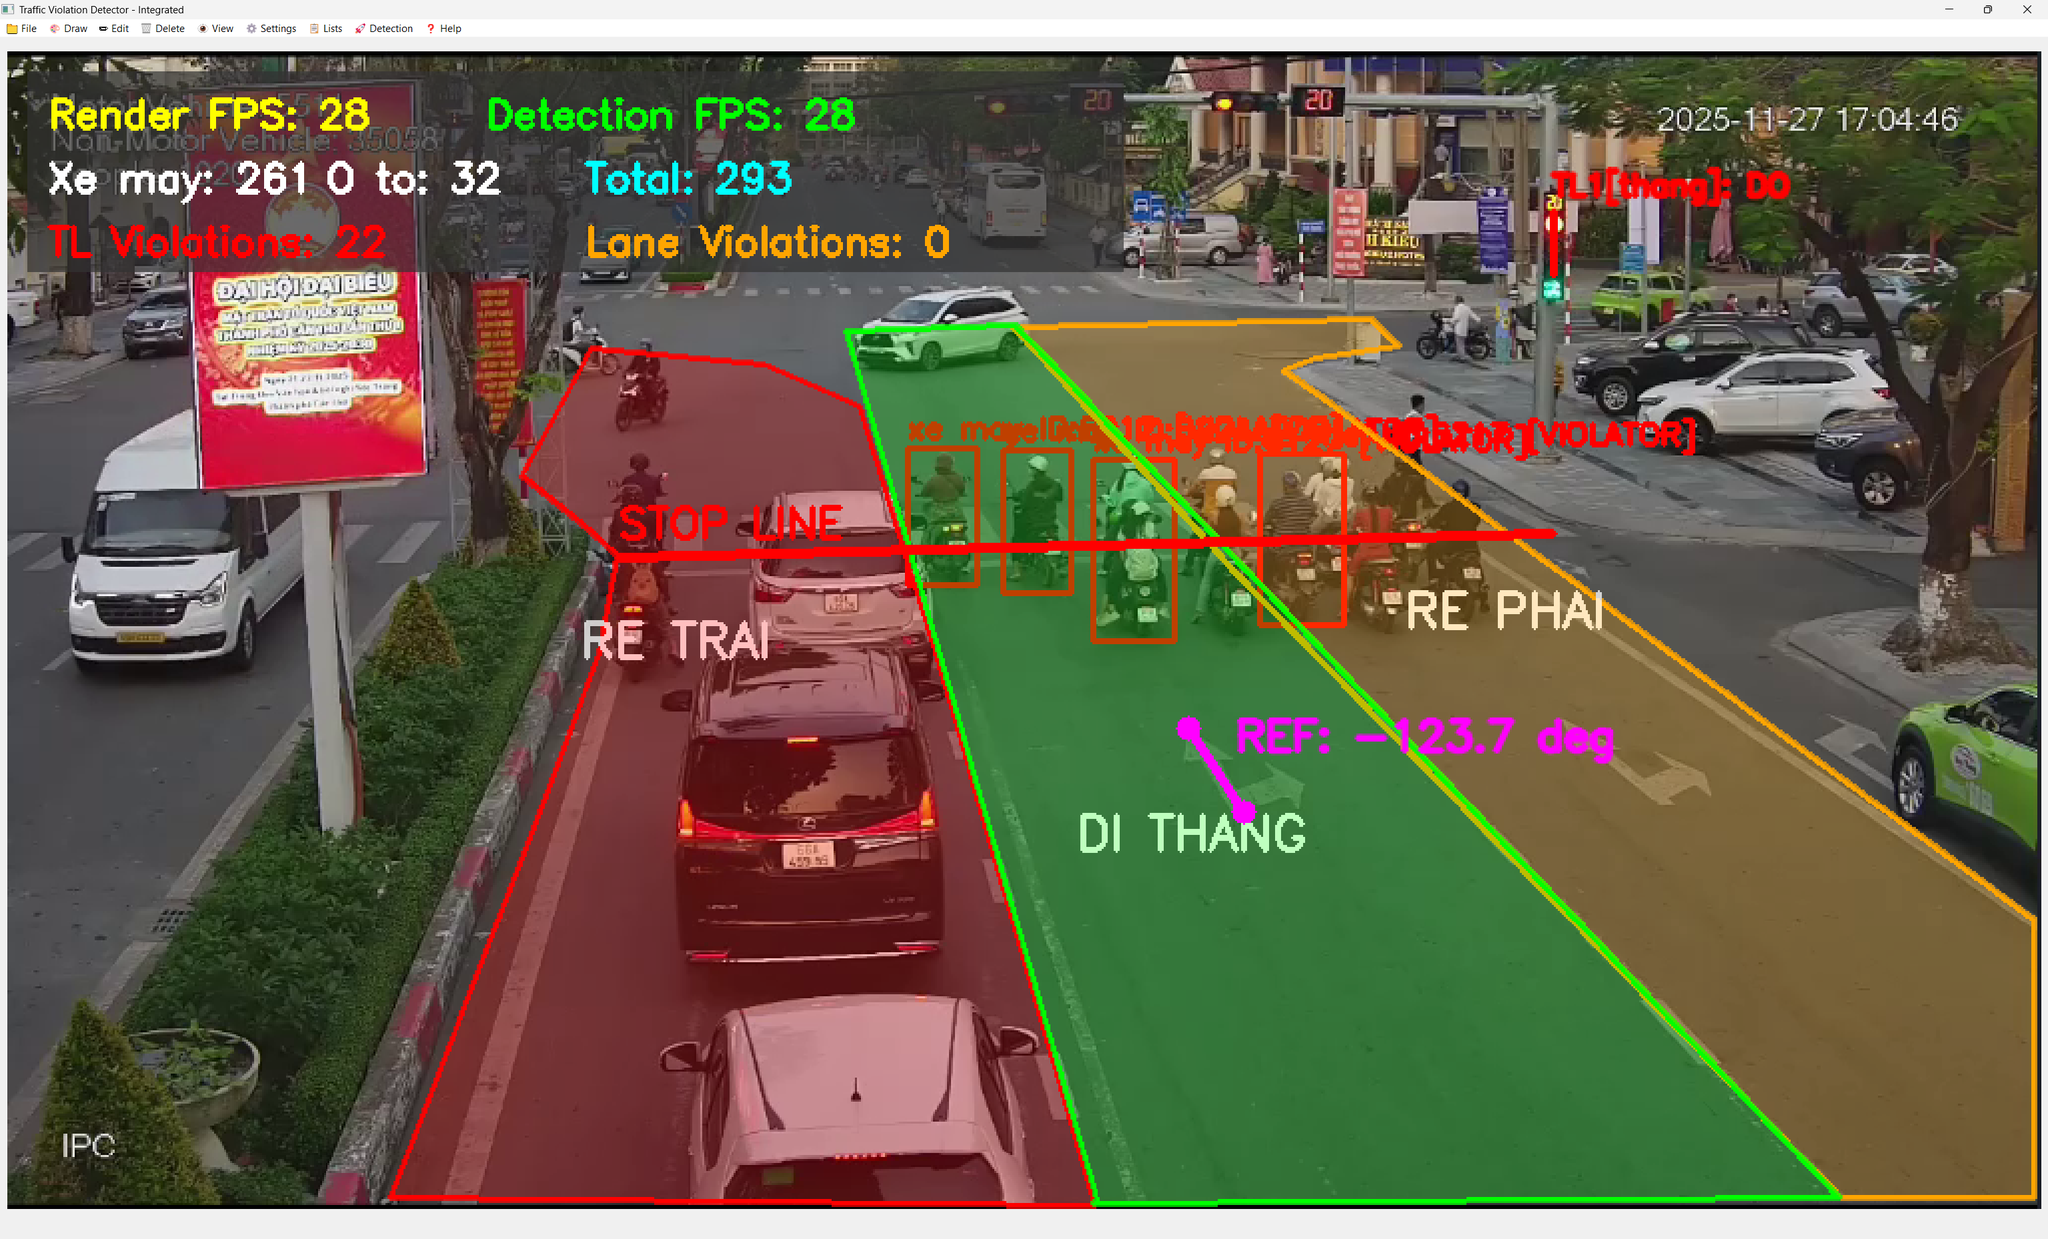
\includegraphics[width=0.7\linewidth]{Figures/inference1.png}
        \caption{Phát hiện xe vượt đèn đỏ (Bbox đỏ = vi phạm)}
    \end{figure}

    \framebreak

    \begin{figure}
        \centering
        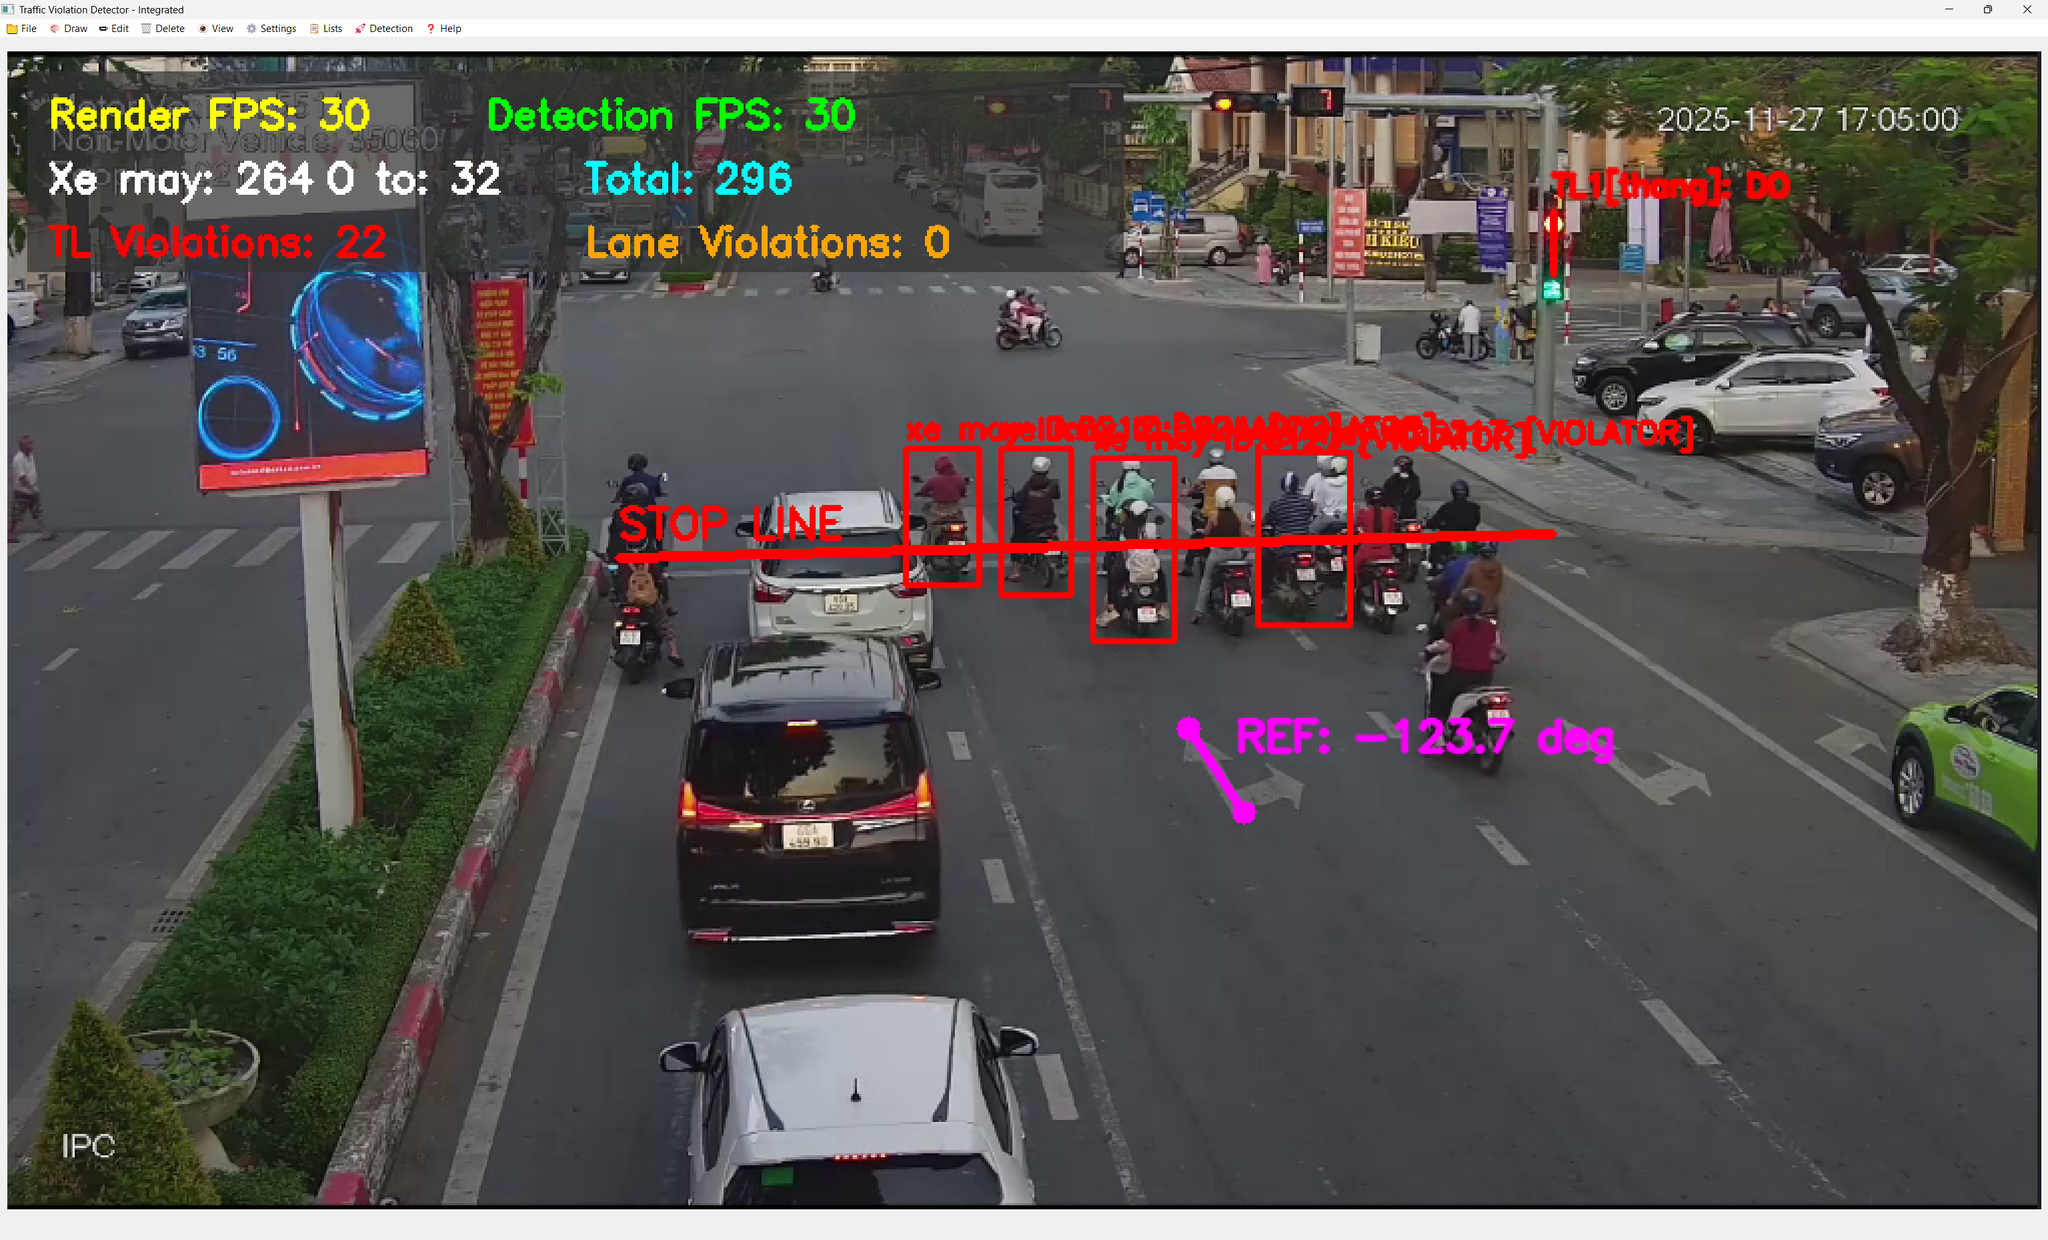
\includegraphics[width=0.7\linewidth]{Figures/inference2.png}
        \caption{Phân loại xe tuân thủ (Bbox xanh) và vi phạm (Bbox đỏ)}
    \end{figure}

    \framebreak

    \begin{figure}
        \centering
        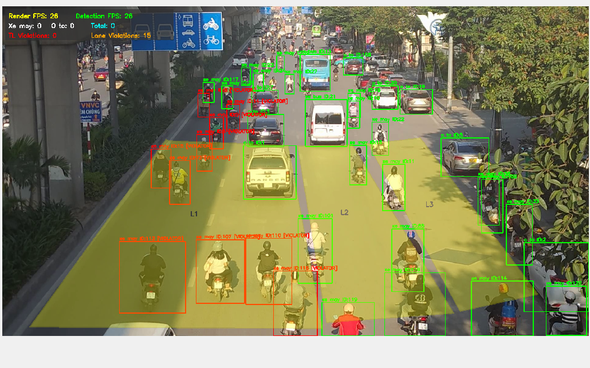
\includegraphics[width=0.7\linewidth]{Figures/inference3.png}
        \caption{Phát hiện xe đi sai làn đường}
    \end{figure}
\end{frame}

%--- ĐÁNH GIÁ HỆ THỐNG ---
\begin{frame}{Đánh giá hệ thống phát hiện vi phạm}
    \begin{block}{Kịch bản 1: Vượt đèn đỏ}
    \begin{itemize}
        \item Logic so sánh tọa độ xe với vạch dừng ảo hoạt động chính xác
        \item Kết hợp với trạng thái đèn (HSV) để đưa ra quyết định
        \item Hỗ trợ 4 loại đèn: Tròn, Rẽ trái, Rẽ phải, Đi thẳng
    \end{itemize}
    \end{block}

    \begin{block}{Kịch bản 2: Đi sai làn}
    \begin{itemize}
        \item Thuật toán Point-in-Polygon xác định xe thuộc làn nào
        \item So sánh loại xe với danh sách cho phép của làn
        \item Hoạt động tốt ngay cả với góc camera thấp
    \end{itemize}
    \end{block}
\end{frame}

%--- THÁCH THỨC VÀ HẠN CHẾ ---
\begin{frame}{Thách thức và Hạn chế}
    \begin{columns}
        \column{0.5\textwidth}
        \textbf{Thách thức đã giải quyết:}
        \begin{itemize}
            \item Mật độ giao thông cao
            \item Điều kiện ánh sáng thay đổi
            \item Đa dạng loại biển số VN
            \item Góc camera nghiêng
        \end{itemize}

        \column{0.5\textwidth}
        \textbf{Hạn chế còn tồn tại:}
        \begin{itemize}
            \item Biển số bẩn/mờ
            \item Biển số nhỏ/xa (Pipeline 2)
            \item Tốc độ giảm khi nhiều xe
            \item Cấu hình ROI thủ công
        \end{itemize}
    \end{columns}
\end{frame}

%--- TỔNG KẾT ---
\begin{frame}{Tổng kết}
    \begin{alertblock}{Kết quả đạt được (theo báo cáo)}
    \begin{itemize}
        \item \textbf{Phát hiện phương tiện:} mAP@50 = \textbf{86.1\%}
        \item \textbf{Phát hiện biển số:} mAP@50 = \textbf{99.5\%} (Pipeline 1)
        \item \textbf{Mô hình tích hợp:} mAP@50 = \textbf{78.5\%} (all classes)
        \item \textbf{Tracking:} ID switches < 5\%
        \item \textbf{Vi phạm:} False positive < 2\%
        \item \textbf{Tốc độ:} 5--20 FPS tùy pipeline
    \end{itemize}
    \end{alertblock}

    \begin{block}{Hướng phát triển}
    \begin{itemize}
        \item Tích hợp auto-retry khi OCR confidence thấp
        \item Hỗ trợ cross-camera tracking
        \item Tự động phát hiện ROI bằng Lane Detection
        \item Triển khai trên edge devices (Jetson)
    \end{itemize}
    \end{block}
\end{frame}

%--- ĐÓNG GÓP ---
\begin{frame}{Đóng góp của đề tài}
    \begin{enumerate}
        \item \textbf{So sánh 2 Pipeline ALPR:}
        \begin{itemize}
            \item Two-Stage: mAP 99.5\%, 5--10 FPS
            \item One-Stage: mAP 78.5\%, 15--20 FPS
        \end{itemize}

        \item \textbf{Huấn luyện 3 mô hình:}
        \begin{itemize}
            \item Model 1: YOLOv8n (5 lớp xe) - mAP 86.1\%
            \item Model 2: YOLOv8n (1 lớp plate) - mAP 99.5\%
            \item Model tích hợp: YOLOv8n (6 lớp) - mAP 78.5\%
        \end{itemize}

        \item \textbf{Hệ thống phát hiện vi phạm:}
        \begin{itemize}
            \item Vượt đèn đỏ (4 loại đèn)
            \item Đi sai làn (Point-in-Polygon)
            \item Direction Fusion (Trajectory + ROI)
        \end{itemize}

        \item \textbf{Ứng dụng:} PyQt5, cấu hình JSON, xuất báo cáo
    \end{enumerate}
\end{frame}

%--- CÂU HỎI ---
\begin{frame}{Câu hỏi thảo luận}
    \centering
    \Huge \textbf{Q\&A}

    \vspace{1em}
    \normalsize
    \textit{Mời thầy cô và các bạn đặt câu hỏi}
\end{frame}


\begin{frame}[plain]
    \centering
    \Huge \textbf{Cảm ơn thầy cô và các bạn đã lắng nghe!}
\end{frame}

\end{document}
